\chapter[Linear ICS at Astra Gemini]{Linear Inverse Compton Scattering at Astra Gemini}
\label{Chap:linICS}
                                                                                                                                                                                                                                                                                                                                                                                                                                                                                    \section{Motivation}

Photons scattering off of a relativistic electron are Doppler-upshifted due to the relativistic Lorentz boost, converting, for instance, optical photons from a laser into X-rays and gamma radiation. This process is called \textit{inverse Compton scattering}, \textit{relativistic Thomson scattering} or \textit{Compton backscattering}.
\textit{Linear inverse Compton scattering} (ICS), the low-intensity limit of this process, is widely used in conventional accelerators as high-energy radiation source to study nuclear processes \cite{Nakano2001_ICSNuclear}, and as versatile beam diagnostic to measure, for instance, the beam energy \cite{Chouffani2006_ICS_BeamParam,Utsunomiya2014_ICS_BeamEnergy}, position \cite{Sakai2002_ICS_LaserWire}, emittance \cite{Sakai2002_ICS_EMITTANCE} and polarisation \cite{Barber1993_POL,Baylac2002_POL,Weber2018_POL}.

More recently, it has also found more application in laser wakefield accelerators (LWFA) \cite{Corde2013_Rad,Albert2016_APP,Downer2018_DiagnosticReview}, for instance, as X-ray source for imaging applications, including high-Z materials \cite{Banerjee2015_ICS_RADIOGRAPHY}. Since the radiation inherits the ultrafast nature of the LWFA electron beam \cite{Lundh2011_BUNCH}, it also has potential as X-ray probe for fast processes like laser-driven shocks in materials \cite{Wood2018_BetatronShock} or structural transitions such as non-thermal melting \cite{Albert2016_APP}.
In the LWFA context linear ICS has also been considered as diagnostic to measure properties of the accelerated electron beam \cite{Jochmann2013_ICS_BeamEAngle,Golovin2016_ICS_BeamEmittance,Kramer2018_Gamma}. 

Typically, at conventional accelerators and in LWFA experiments the beam is diagnosed by scanning or rastering the laser over multiple shots through the electron beam (see `laser wire' \cite{Alley1996_LaserWire,Leemans1996_ICS_BeamTransLong,Sakai2001_BeamSize,Sakai2002_ICS_LaserWire,Honda2005_ICS_LaserWire}). In all-optical setups the laser is then focused tightly in order to produce a significant number of X-rays or gamma-rays \cite{Kramer2018_Gamma}. In conventional accelerators the typical beam charges are much higher such that Fabry-Perot cavities excited by a continuous-wave laser can be used \cite{Honda2005_ICS_LaserWire}. A statistical characterisation of the electron beam is only meaningful if the beam source is either reproducible, as in conventional setups, or particle beam transport is used to focus the electron bunch onto a fixed point in space. The performance of LWFA sources has in the recent years greatly improved \cite{Mangles2016_LPA_Review}, also in terms of reproducibility and repetition rates, which is also a key development target to be competitive with other light sources \cite{Albert2016_APP}.

A sufficiently intense laser pulse, on the other hand, can produce a significant yield of scattered photons at a large beam diameter comparable to the size of the electron beam or exceeding it. 
In such a setup the Compton source could act as single-shot diagnostic similar to a beam profile monitor, measuring electron beam pointing, divergence and ellipticity, and their statistical fluctuations. The same setup can then be used at high intensities in nonlinear ICS where the ellipticity of the emission profile has been proposed as on-shot intensity measurement of the interaction \cite{HarShemesh2012_INTENSITY,Yan2017_ICS,Blackburn2019_ModelIndependentLaser}. A statistical characterisation of the electron beam would be a useful tool to discriminate variations in the electron beam and the gamma ray emission and, as a result, separate model uncertainties related to radiation reaction and the emission profile from experimental uncertainties caused by the intrinsic fluctuations of the laser wakefield accelerator.

\section{Chapter Outline}

This Chapter presents results from an experimental experimental campaign undertaken at the \textsc{Gemini} laser system in early 2019, aimed at conducting precision measurements of radiation reaction by colliding highly relativistic electron beams from laser wakefield acceleration with an intense laser pulse. Unfortunately, losing access to the scattering laser beam towards the end of the campaign due to a damaged component in the laser beam line, we were not able to perform interactions at high-intensities. We, however, succeeded in colliding a relativistic electron beam with a defocused laser pulse at $a_0 \sim 0.2-1.0$ over the course of hundreds of shots, and in measuring the emitted high-energy radiation from linear inverse Compton scattering produced in the process. In this Chapter we demonstrate how to use the properties of the emitted radiation to diagnose the scattering laser pulse and the electron beam.

After outlining the experimental layout of the campaign, we proceed with a characterisation of the electron spectra taken at fixed experimental conditions (Section \ref{Chap:linICS:sec:Espec}). These electron beams were interacted with the laser pulse to act as Compton source. 

Then results from a laser raster scan are presented (Section \ref{Chap:linICS:Sec:RasterScan}): by shifting the scattering beam relative to the electron bunch and measuring the presence or absence of a bright gamma signal on the gamma profile detectors, the size of the laser beam at the interaction plane was established. Here, the electron beam is small and approximately fixed in space so that it acts as a probe rastering the laser beam profile. This technique can be used to corroborate the spatio-temporal electron-laser alignment and estimate the required change in the relative arrival time of those to achieve high-intensity interactions.

Based on the estimated laser beam parameters at the interaction and the characterised electron beams, the spectral shape of the produced radiation is discussed (Section \ref{Chap:linICS:Sec:GammaSpec_A}), followed by an estimate of the total number of high-energy photons produced in the interaction (Section \ref{Chap:linICS:Sec:Nphotons}) and how different spectral components of the electron beam contribute to the total yield measured on the scintillating profile screen used in the experiment (Section \ref{Chap:linICS:Sec:EdepResponse}).
The photon yield is used to infer the beam size and intensity at the interaction point (Section \ref{Chap:linICS:Sec:YieldBeamSize}), and could be used to diagnose the temporal fluctuations in the synchronisation of the laser pulse and the electron beam. Subsequently, the spectrum of the emitted radiation is inferred for specific example shots (Section \ref{linICS:Chap:Sec:SpectralRetrieval}).

Finally, the feasibility of this light source as single-shot non-invasive electron beam diagnostic is discussed, in particular its ability to measure the beam divergence, pointing and to resolve spatial features of the electron beam (Section \ref{Chap:linICS:Sec:ICS_EbeamDiag}). 

\section{Experimental Setup}
\label{Chap:linICS:sec:ExpSetup}

This experiment was performed at the \textsc{Gemini} facility in early 2019 using both laser arms of the dual laser beam facility.
A sketch of the relevant components of the setup is shown in Figure \ref{LinICS:Fig:SetupBlend}.

\subsubsection{Laser wakefield accelerator}

The driver beam for the wakefield accelerator was focused by an $f/40$ off-axis parabola (OAP) onto the leading edge of a 15 mm conical supersonic helium gas jet. The measured pulse duration was $61\pm5\,\mathrm{fs}$ \textsc{fwhm} with an average energy on-target of $12.5 \pm 0.2\,\mathrm{J}$, reaching a peak power of $195\pm3\,\mathrm{TW}$. The size of the focal spot measured $(48.6\pm3.2) \times (39.2\pm1.6)\,\mathrm{\upmu m}$ \textsc{fwhm}, amounting to a peak normalised vector potential of $a_0 = 1.88\pm0.04$ in vacuum\footnote{The focal spot data and FROG trace were analysed by Matthew Streeter (Imperial College)}. The laser pulse was polarised in the horizontal plane.
\vspace{\baselineskip}

The exit of the gas nozzle was positioned $14\pm0.1\,\mathrm{mm}$ below the laser beam axis to avoid damage from the second, more divergent laser beam. A steel razor blade was introduced $4\pm0.1\,\mathrm{mm}$ above the nozzle edge at $- 32.4^\circ\pm 0.3^\circ$ angle in vertical direction relative to the laser axis to produce a shock front. The tip of the blade was inserted $1.2\pm0.1\,\mathrm{mm}$ into the gas flow from the same side that the driver beam entered from. 
The gas target was characterised on-shot by a transverse optical probe synchronised with the driver beam ending in a shadowgraphy and a Mach-Zehnder interferometry setup.
The interferometrically determined electron density\footnote{The interferometry data was evaluated by Cary Colgan (Imperial College)} without inserting the blade was $(1.4 \pm 0.2) \times 10^{18}\,\mathrm{cm}^{-3}$. When inserting the blade the density profile exhibited a sharp peak in density reaching about $(2.4 \pm 0.2) \times 10^{18}\,\mathrm{cm}^{-3}$, which is about twice the ambient density.
In addition to the optical probe, the gas target and the recombination light emitted by the plasma channel were imaged by a Canon DSLR camera from the side and a CCD camera from the roof of the chamber.

\begin{figure}
\centering
\includegraphics[width=0.9\columnwidth]{GeminiShock2019_ExpBlend_V1_Aug20_annotated.png}
\caption[Sketch of experimental setup to measure radiation from linear inverse Compton scattering.]{Sketch of the experimental setup aimed to measure radiation from linear inverse Compton scattering. The first laser pulse (red, left) is focused down by an $f/40$ OAP into a gas jet and accelerates electrons (blue) from LWFA, where the density perturbation induced by the blade affects the injection mechanism. A second laser is focused down by an $f/2$ OAP and counter-propagates with the electron beam performing linear inverse Compton scattering. Gamma radiation produced in the interaction (green) is emitted in the propagation direction of the electron beam and is measured downstream by a scintillating profile screen and a stack of scintillating crystals used as spectrometer (right). A converter target behind the $f/2$ OAP can be used to convert the electron beam via bremsstrahlung into an energetic calibration source for the gamma diagnostics. The electrons are dispersed horizontally by a permanent dipole magnet onto a set of Lanex screens. The accelerator, the interaction point and the magnet are in vacuum, whereas the measurement screens and gamma diagnostics are located at air separated by a thin vacuum window (orange).} 
\label{LinICS:Fig:SetupBlend}
\end{figure}
\subsubsection{Scattering beam}

A second laser pulse was focused by an $f/2$ off-axis parabola (OAP) at the opposite edge of the gas jet in a head-on geometry. The $f/2$ OAP had a 21-mm-diameter hole in the centre that allowed the electrons, laser light and radiation on-axis to propagate through. A plastic ring of outer radius $28\,\mathrm{mm}$ and inner radius $11\,\mathrm{mm}$ was fitted around the hole to protect the optic and the laser chain upstream from laser light that was potentially scattered or strongly defocused in the plasma. This reduced the energy on-target by 16 percent assuming a perfect top-hat laser profile and that the collimated beam incident on the OAP had a diameter of $150\,\mathrm{mm}$. To protect the optic from potential debris a thin plastic layer with anti-reflective coating (`pellicle') and a suitable hole was attached to the mount of the OAP. The on-shot energy of the laser after the compressor was $9.73\pm 0.15\,\mathrm{J}$ and $8.17\pm0.13\,\mathrm{J}$ on-target due to the hole in the OAP. In the dataset presented, the beam diameter at the interaction was estimated to be $400\pm100\,\mathrm{\upmu m}$, which translates into $a_0 \sim 0.28 \pm 0.04$ at a pulse duration of $45\,\mathrm{fs}$. The laser pulse was linearly polarised in the vertical plane, cross-polarised to the wakefield driver beam.

\subsubsection{Two-beam timing}

Both laser beams were synchronised to each other in vacuum to an accuracy of $\pm30\,\mathrm{fs}$ using spatial interferometry \cite{Cole2018_RR}. A 90-degree dielectric knife-edge prism (Thorlabs MRAK25-E03) was inserted at the interaction point, deflecting both beams collinearly onto the CCD chip of a camera (AVT Manta G-033B) equipped with a $\times10$ long-working-distance infinity-corrected microscope objective (Mitutoyo NIR). Due to the different radii of curvature of both beams, especially near the focus of the $f/2$ beam, a circular interference pattern emerged when the beams were overlapped in space and time. The timing procedure is explained in more detail in Section \ref{Methods:Sec:DualBeamTiming} of the \nameref{Chap:Methods} Chapter.

\subsubsection{Particle and Radiation diagnostics}

The radiation, the remaining driver laser and the electrons propagated through the hole in the $f/2$ OAP into a large aperture [$10\,\mathrm{cm} \times 30\,\mathrm{cm}$ (vertical $\times$ horizontal)] permanent dipole magnet\footnote{designed, and assembly and positioning supervised by Dominik Hollatz (Jena)} of integrated magnetic field strength $\int B(x) \mathrm{d}x = 0.35\,\mathrm{Tm}$. 
The electrons were dispersed in the horizontal plane and electrons of energy lower than 220 MeV collided with the yoke of the magnet resulting in an effective low-energy cut-off. The dispersed beam left the vacuum chamber through a two-layer wide-aperture vacuum window\footnote{designed and tested by the Mechanical Engineering Division at the CLF, in particular Daniel Treverrow.} of dimensions $580 \,\mathrm{mm} \,\times\, 70\,\mathrm{mm}$ (horizontal $\times$ vertical). The layer facing the vacuum consisted of $25\,\mathrm{\upmu m}$ of Kapton, the outside layer is $375\,\mathrm{\upmu m}$ of Kevlar (chemical equation $C_{14} H_{14} N_2 O_4$, density $\rho = 1.44\,\mathrm{g/cm}^3$ \cite{Kevlar}) providing additional mechanical stability and fibre support that acted as mechanical fail-safe. A scintillating sensitive Lanex screen (Kodak Biomax) was placed just after the window, at $1.61\,\mathrm{m}$ distance downstream of the interaction point, to measure the spectrum of the dispersed electron beam. The screen also extended beyond the laser and radiation axis. The light and thin material of the window and the short distance to the Lanex screen minimised the impact of multiple small-angle scattering on the measurement \cite{Moller1932_Moller,Bethe1953_Moliere}.
A second Lanex screen (Kodak Standard) measured the spectrum $700\pm1\,\mathrm{mm}$ further downstream ($2.31\,\mathrm{m}$ from the interaction point) and can in conjunction with the first screen be used to account for the pointing of the beam \cite{Clayton2010_ION,Soloviev2011_TWOSCREEN}.
The screens were each imaged by a cooled 16-bit CCD camera (Andor Neo) equipped with a suitable objective and a bandpass filter transmitting light of wavelength $546\pm10\,\mathrm{nm}$. %A third camera images a small region of interest on the first screen.
\vspace{\baselineskip}

High-Z metal converter targets (bismuth, tungsten, iron) were fixed to a $1.6\,\mathrm{mm}$ plastic (PTFE) base and mounted on a motorised linear stage between the mount of the $f/2$ OAP and the dipole magnet. The targets were driven into the beam path to intercept the electron beam and to produce gamma radiation from bremsstrahlung \cite{Glinec2005_Brems} to calibrate the gamma-ray diagnostics in this experiment \cite{Behm2018_Gamma}. The high-Z targets enabled efficient conversion of the electron beam energy into radiation, but did not allow measuring the electron spectrum at the same time. The PTFE base itself was also used as converter that was less efficient in terms of radiation yield but allowed a synchronous measurement of the electron and gamma-ray beam. 

Radiation traversed the magnet on the laser axis, then passed through a $120\,\mathrm{\upmu m}$ aluminium laser beam block terminating the wakefield driver beam, and the Kevlar-Kapton window mentioned before. Bright radiation in the right bandwidth was also captured by the Lanex screen as it extended beyond the laser and radiation axis. An array of $45 \times 45$ scintillating with thallium doped caesium-iodide (CsI:Tl) crystals of dimensions $1\,\mathrm{mm} \times 1\,\mathrm{mm} \times 10 \,\mathrm{mm}$ measured the profile of the radiation $700 \pm 1\,\mathrm{mm}$ downstream from the plane of the first Lanex screen. The crystals were each separated transversely by a $0.2\,\mathrm{mm}$ thick $TiO_2$ coating and were held together by a $TiO_2$ front plate of thickness $0.5\mm$. The stack covered a field of view corresponding to a cone of half opening angle $11.7\,\mathrm{mrad}$. The spatial resolution including the coating separating the individual crystals was then $1.2\,\mathrm{mm}/2.31\,\mathrm{m} = 0.52\,\mathrm{mrad}$.
$704 \pm 1\,\mathrm{mm}$ further downstream from the profile screen another elongated array of caesium-iodide crystals was positioned to measure the spectrum of the gamma radiation. Both scintillator arrays, the profile screen and the spectrometer, were imaged using cooled 14-bit EMCCD cameras (Andor iXons). The diagnostics are described in more detail in Section \ref{Methods:Sec:GammaDiags}.

\section{Characterisation of Electron Spectra}
\label{Chap:linICS:sec:Espec}


\begin{figure}
\centering
\includegraphics[trim={4.0cm 0 3cm 0}, clip, width=1.0\columnwidth]{Example_Montage_twoSets_V2.png}
\caption[Waterfall plot for electron spectra at fixed conditions.]{Waterfall plot of electron spectra measured at fixed experimental conditions. The y-axis indicates the electron energy in MeV, the x-axis shows the order the shots were taken in. The electron spectra measured on the Lanex screens were integrated in the non-dispersion axis and each occupy one column in this waterfall plot. The colour scale indicates the charge per MeV in the beam.}
\label{linICS:Figs:fixed_waterfall}
\end{figure}

In this experiment the electrons were injected through density perturbations in the supersonic gas flow which were introduced by a steel blade \cite{Schmid2010_SHOCK} and subsequently accelerated to relativistic energies via laser wakefield acceleration (LWFA). The electron spectrum was measured by scintillating Lanex screens as part of a magnetic spectrometer setup. Details of the diagnostic and the relevant image processing of the data can be found, for instance, in \cite{ColeThesis,PoderThesis} and Section \ref{Chap:Methods:Sec:Espec}. Here we will only consider the measurements from the first Lanex screen and ignore potentials errors in the inferred electron energy resulting from pointing fluctuations \cite{Clayton2010_ION,Soloviev2011_TWOSCREEN}.

We consider a dataset consisting of a series of shots taken at fixed experimental conditions, which allows investigating fluctuations in the accelerator performance. The electron beams measured on these shots were collided with a second laser pulse to produce radiation from inverse Compton scattering, which will be analysed in more detail in the following sections.
The dataset consists of 386 shots on which electron beams were measured, taken at constant backing pressure of the gas jet and fixed blade position ($1.2\pm0.1\,\mathrm{mm}$ into the gas flow from the entry point of the driver beam). A waterfall plot of the in non-dispersion direction integrated 1D electron spectra is shown in Figure \ref{linICS:Figs:fixed_waterfall}. Despite the constant conditions, the properties of the electron beams vary strongly from shot-to-shot and beams of a wide range of shapes, maximum energy and energy spread are measured. A few examples of the 2D electron spectra from the dataset are provided in Figure \ref{linICS:Figs:Elec_example}.
The spectral bandwidth of the beams varies strongly with some exhibiting an almost flat spectrum spanning hundreds of MeV (see 4 left panels in Figure \ref{linICS:Figs:Elec_example}). These spectrally very wide electron beams show signatures of strong transverse oscillations which indicate their potential to act as a bright betatron source \cite{Corde2013_Rad}. In other instances electron beams with narrow energy spread around $1\,\mathrm{GeV}$ are measured (right panels in Figure \ref{linICS:Figs:Elec_example}). 

\begin{figure}
\centering
\includegraphics[trim={4cm 0 1cm 0}, clip, width=1.0\columnwidth]{Example_Espec_CollisionMontage_V3.png}
\caption[Examples of 2D electron spectra measured in the experiment.]{Examples of 2D electron spectra measured in the experiment. The y-axis is the dispersion axis and shows the electron energy in MeV on a linear scale, the x-axis indicates the divergence in mrad. The colour scale indicates the amount of charge per MeV per mrad in the beams and is fixed for all plots. Projections of the beams are shown on the respective axes: on the x-axis the over the dispersion-axis integrated spectrum is shown and is equivalent to the horizontally integrated spatial profile of the beam and is shown as charge per mrad as a function of divergence in mrad. The projection on the y-axis is the in non-dispersion axis integrated spectrum as also shown in the waterfall plot in Figure \ref{linICS:Figs:fixed_waterfall} and shows the charge per MeV as a function of the electron energy in MeV. The amplitude of the projections is fixed across all panels and is not representative of the relative charge between the panels.}
\label{linICS:Figs:Elec_example}
\end{figure}

The striking variability of the electrons produced in this dataset at seemingly fixed experiment conditions is not consistent with experimental results reported from other LWFA experiments at other laser systems using shock injection \cite{Schmid2010_SHOCK}. These setups typically provide reproducible electron beams with narrow energy spread \cite{Schmid2010_SHOCK,Buck2013_SHOCK,Swanson2017_SHOCK,Tsai2018_SHOCK}. 
\vspace{\baselineskip}

\begin{figure}
\centering
\includegraphics[trim={5cm 0 6cm 0}, clip, width=1.0\columnwidth]{linICS_ElectronProperties_Histograms_V3.png}
\caption[Histogram of fluctuations in the electron beam properties in this dataset.]{Histograms showing the fluctuations of electron properties in course of this dataset (386 shots). Top left: Total charge of the electron beams measured from 220 MeV upwards. Top right: Maximum electron energy, defined as energy at which the spectral intensity falls to 10 percent of its peak value. Bottom left: vertical divergence (non-dispersion axis, \textsc{fwhm}) in mrad. Bottom centre: Beam pointing fluctuation in mrad from the mean position. Bottom right: On-shot laser energy of the wakefield driver beam in Joules.}
\label{linICS:Figs:Elec_histogram}
\end{figure}

The key properties of the electron beams in this dataset are summarised in Figure \ref{linICS:Figs:Elec_histogram} in form of histograms showing charge, maximum electron energy, vertical (non-dispersion axis) divergence, beam pointing and on-shot laser energy of the wakefield driver beam.
The maximum energy of the electron beam, here defined as the energy when the spectral intensity reaches 10 percent of its peak value, measured on average $944\pm139\,\mathrm{MeV}$ (error indicates standard deviation based on normal distribution), with some shots reaching up to $1.3\,\mathrm{GeV}$. The charge of the beam varied in particular due to the varying spectral range of the bunch with a median of $225(+67/-56)\,\mathrm{pC}$, where the error interval indicates the quarter and three quarter quantile, respectively, as the distribution is not normal.
The divergence of the beams was measured to be $2.1(+0.6/-0.5)\,\mathrm{mrad}$, again indicating the quarter, median, and three quarter quantile, and the vertical position of the beam centroid was fluctuating by $2.2\,\mathrm{mrad}$, assuming a normal distribution. The on-shot laser energy was on average $12.3\pm0.5\,\mathrm{J}$, assuming a normal distribution. The linear correlation coefficient for the laser energy and the maximum electron energy is $0.03$ which indicates that the quantities are not correlated. This is consistent with shock injection where the position of the density perturbation, the injection point, determines the maximum energy, and also indicates that the injection point varies from shot to shot, potentially due to a variation in the shock position and angle. The charge in the beam is only moderately correlated with the laser energy at a coefficient of $0.29$.
\vspace{\baselineskip}

The wide range of electron beams produced in this setup is interesting in the context of radiation production by linear inverse Compton scattering (ICS). Since the properties of the beams this accelerator generates vary strongly, the radiation these electron beams are capable to produce in a well-defined linear ICS interaction will also vary significantly. This means that this accelerator is in principle also able to produce a wide range of radiation spectra from broadband to strongly peaked radiation, but an increased control over the accelerator would be required to shape the spectral emission and develop a tunable radiation source that can be optimised for a respective application. An improved stability of the shock position could facilitate this control.

\section{Laser raster scan}
\label{Chap:linICS:Sec:RasterScan}
\begin{figure}[h]
\centering
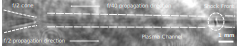
\includegraphics[width=0.8\columnwidth]{RasterScan_Shadowgraphy_CloseUp_annotated.pdf}
\caption[Shadowgram of the plasma channel with the focusing f/2 laser cone.]{Cut-out of a shadowgram of the gas jet taken with the transverse optical probe (horizontal plane). The wakefield driver beam enters the gas jet from the right side and generates a plasma channel. The dark line on the right side results from a shock front. The second scattering beam is focused tightly into the plasma from the left side, where a converging cone becomes visible. The spatial scale is indicated in the bottom right corner.}
\label{linICS:Figs:ShadowgraphyRaster}
\end{figure}


The laser pulses from the two laser arms were overlapped in space and time using a photodiode and spatial interferometry in vacuum (see Section \ref{Methods:Sec:DualBeamTiming}). The focal plane of the scattering $f/2$ beam was positioned in the gas jet for alignment purposes. On full-power shots the cone of the $f/2$ laser pulse focusing into the plasma is visible on the transverse (horizontal plane) shadowgraphy diagnostic (see Figure \ref{linICS:Figs:ShadowgraphyRaster}, left side) along with the plasma channel from the wakefield driver beam and the shock leading to the injection of electrons into the wakefield accelerator (dark line in the plasma channel on the right side). 
\vspace{\baselineskip}

On full-power shots with both laser beams and an electron beam produced by the wakefield accelerator, we consistently measured a bright circular or oval signal on the gamma profile screen indicating an interaction of the laser pulse and the electron beam (inverse Compton scattering). 
The consistency of the collisions implies that the laser beam is much larger than the electron beam, and the combined fluctuations in the relative position of the scattering beam and the electron beam. 
This in turn indicates a systematic offset of the interaction point from the focal plane of the $f/2$ laser pulse that we attempted to achieve with the alignment and timing procedure, as the laser pulse and the electron bunch would there be of comparable size and are expected to miss each other frequently \cite{Cole2018_RR}.

\begin{figure}
\centering
\includegraphics[trim={8cm 2.5cm 6cm 2.5cm}, clip, width=1.0\columnwidth]{linICS_RasterScan_GammaProfile_Montage_V3.png}
\caption[Montage of gamma profile measurements taken during an OAP raster scan.]{Montage of gamma profile measurements at different transverse OAP positions. Each panel shows a the measured gamma profile images for a series of shots taken at a fixed OAP position. The panels are labelled with the relative transverse offset of the OAP for that particular dataset. The colour scale indicates the measured yield of scintillation light which is proportional to the energy deposited in the profile stack, but is not constant across the panels.}
\label{linICS:Figs:GammaProfileRaster}
\end{figure}


To establish the transverse size of the scattering laser pulse at the interaction point, the scattering laser beam was shifted horizontally by translating the position of the $f/2$ off-axis parabola (OAP) in $50\,\mathrm{\upmu m}$ steps, assuming that the laser beam translates by the same amount for small motions. 
The remaining experimental parameters and the alignment of the wakefield driver beam were kept constant during this procedure. 
At each OAP position at least 5 full-power dual-beam shots were taken. In some cases, if at least one of the lasers was not firing or no electron beam was measured on-shot, additional shots were required in order to accumulate 5 suitable data points at each OAP position. The response of the gamma profile screen was recorded and the number of visible bright signals was noted down. Subsequently, the OAP was then translated again by $50\,\mathrm{\upmu m}$ and the procedure was repeated. Figure \ref{linICS:Figs:GammaProfileRaster} shows a montage of the gamma profile screens at each position of a horizontal scan in the OAP position, where the relative position from the established beam centre is indicated on the $x$-axis. Figure \ref{linICS:Figs:GammaProfileRasterCounts}, on the other hand, shows the corresponding average integrated gamma yields on the profile screen and the fraction of successful collisions at each position. The absence of bright signals at two two consecutive OAP positions was deemed to be a suitable indication of lacking overlap of the laser beam and the electron bunch. The distance mapped by this method includes the diameter of the laser beam at the plane of the interaction, the size of the electron beam, and the relative pointing fluctuations between them. Since the finite step size in the OAP translation ($50\microns$) is much larger than the expected electron beam size $\sim\microns$ and the relative pointing fluctuations ($\sim \mrad \times \mathrm{mm}$), the dominant measurement error on the transverse size of the laser beam is the step size.


\begin{figure}
\centering
\includegraphics[trim={4cm 0cm 2cm 0cm}, clip, width=0.9\columnwidth]{linICS_RasterScan_GammaProfile_Counts_V2.png}
\caption[Average integrated pixel counts and successful collisions at each OAP position of the laser raster scan.]{Green: Average integrated pixel counts on the gamma profile screen as a function of the relative OAP position. The error bars indicate one standard deviation from the mean based on a normal distribution. Blue: Fraction of successful collisions at each OAP position. The grey dashed lines indicate the determined beam size.}
\label{linICS:Figs:GammaProfileRasterCounts}
\end{figure}

In the raster scan presented in Figure \ref{linICS:Figs:GammaProfileRaster} and Figure \ref{linICS:Figs:GammaProfileRasterCounts} the interaction region and hence, following our argument, the combined size of the laser beam and the electron beam along with variations in the relative beam pointing was $400\pm100 \,\mathrm{\upmu m}$. 
The integrated gamma yield in Figure \ref{linICS:Figs:GammaProfileRasterCounts} also shows signs of a drop in intensity throughout the scan, potentially when crossing the hole in the beam. 
At an energy on-target of $9.73\pm0.15\,\mathrm{J}$ this amounts to an average $a_0 \approx 0.28 \pm 0.04$, where we assumed a perfect flat-top beam profile and hence ignored the reduction of the energy in the beam due to the hole in the $f/2$ OAP as this does not affect the local photon density in the near-field. 
For an $f/2$ geometry this also indicates that the interaction occured at $\sim1.1\pm0.1\,\mathrm{mm}$ distance from the focal plane. 
Based on the alignment procedure in the experiment we suspect that the interaction occurs prior to the focus of the scattering beam (left hand side in Figure \ref{linICS:Figs:ShadowgraphyRaster}). 
The interaction occurs in the plasma, so that the electron beam is only $\sim \mathrm{\upmu m}$ in size \cite{Weingartner2012_BUNCH} and spatial fluctuations due to pointing variations of the laser with a varying off-axis distribution due to betatron oscillations with betatron amplitudes of typically $r_\beta \sim \mathrm{\upmu m}$ \cite{Corde2013_Rad}. 
Since the beam pointing of the $f/2$ beam is demagnified due to the short focal distance, the raster scan mainly reflects the dimensions of the scattering beam and this is hence a suitable method to determine the size of the laser beam.

If we assume that this method successfully determines the size of the laser pulse at the interaction plane, we can also pinpoint its centre by shifting the OAP to the central position between the outermost OAP positions on which a significant gamma signal was measured. 
By repeating this procedure in the vertical we can accurately centre the scattering laser pulse on the electron beam in both transverse dimensions, provided that the relative pointing fluctuations and the electron beam size are negligible as assumed. 
The accuracy of this procedure can be improved by repeating the steps in the first transverse dimension in a third pass and by reducing the step size of the OAP translation. 
The principle of this `raster scan' resembles the `laser wire' or spatial cross-correlation technique where a scattering laser beam is focused tightly onto an electron beam to produce energetic from linear inverse Compton scattering and to diagnose the electron beam \cite{Alley1996_LaserWire,Leemans1996_ICS_BeamTransLong,Okugi1999_WireScanner_Emittance,Sakai2001_BeamSize,Sakai2002_ICS_LaserWire,Honda2005_ICS_LaserWire,Chen2013_ICS,Jochmann2013_ICS_BeamEAngle,Golovin2016_ICS_BeamEmittance,Kramer2018_Gamma}. The laser focus is typically smaller than the electron beam and the transverse size of the electron beam can be determined by translating the laser focus over multiple shots. The emission spectrum and angular distribution of the backscattered radiation can also be used as diagnostic for other beam properties. The name `laser wire' is derived from the physical wire scanners that were used as beam diagnostics in conventional accelerator facilities \cite{Okugi1999_WireScanner_Emittance}. In the case presented here, the electron beam, however, is much smaller than the laser beam. Even though the laser pulse is translated and the electron remains approximately fixed, here the electron beam effectively acts as the probe and diagnoses the laser beam at the interaction plane, inversely to the laser wire.

Finally, we have to consider that significant translation of the focusing OAP might introduce astigmatism to the laser pulse and we have to optimise the OAP angle and position accordingly.


\iffalse
The gas jet expands from its nozzle opening diameter of $15$ mm to a length of approximately $17.3$ mm (measured by the length of the plasma channel on the shadowgram). This means based on this scan the interaction point is defined as intended by the alignment procedure, the inner edge of the gas nozzle, but the gas jet has expanded. In addition, the focal plane of the laser has changed. We have to keep in mind that translating the OAP in longitudinal direction does not change the intensity of the interaction at first order as we shift the interaction plane along with the intensity plane when doing so. If we want to change the intensity at the interaction we have to change the relative delay of the two laser pulses.
In brief, shifting the longitudinal OAP position and the focal plane in space only changes the plane of interaction at roughly the same intensity, whereas shifting the delay of the beams shifts both the interaction plane and the intensity. The mismatch of the interaction plane and the focal plane might be due to a misunderstanding of these two mechanisms and we mistakenly `compensated' for the shift in focus and fixed the interaction plane, rather than the intensity at the interaction.
\SMComm{Confirm with Matt and Brendan whether this makes sense and matches their memory.}
\fi

\begin{figure}
\centering
\includegraphics[trim={4.5cm 0 5cm 0}, clip, width=.9\columnwidth]{linICS_Raster_WaistSize_V3_annotated.png}
\caption[Sketch of a (2D) laser raster scan.]{Sketch of a (2D) laser raster scan. The laser waist size (red) is shown as a function of the distance from the focal plane, z = 0. The laser is translated in space such that electron beam interacts with a different part of the laser pulse (boxes). If the electron beam intersects the laser pulse energetic radiation from inverse Compton scattering is emitted (green boxes). If the laser pulse and the electron miss each other no radiation is produced (red boxes with crosses). By adjusting the relative time of arrival between the driving laser pulse and the scattering beam the plane of the interaction is shifted (dashed blue lines) and the procedure can be repeated.}
\label{linICS:Figs:RasterTemporalTranslationIdea}
\end{figure}

\subsubsection{Laser raster scan as tool to achieving high-intensity interactions}

By using this spatial correlation technique we can determine the size of the beam at the interaction, its centre and, knowing the focusing geometry, the plane of the interaction. As a result, we can not only characterise the properties of the beam at the interaction, but we can use this information to change the relative time of arrival of both laser pulses to shift the interaction towards a more intense region of the focusing beam. The procedure can then be repeated at the new interaction plane to confirm that the laser pulse is indeed smaller and more intense. This procedure is visualised for a 2D scan in a sketch in Figure \ref{linICS:Figs:RasterTemporalTranslationIdea}. When the beam size of the scattering laser pulse and the electron bunch become comparable, we also expect not only particularly bright gamma-ray yield due to the high laser intensity but also more frequent `missed' shots when the laser pulse and the electron beam pass by each other as the pointing fluctuations are comparable with their sizes.

If we perform this raster scan at a high resolution (small step size) in both transverse dimensions, at various focal planes (multi-dimensional raster scan) and with multiple shots at each position, we immediately see that this requires a large number of shots in total. A route to reducing the number of required shots to identify the ideal high-intensity conditions is using a Bayesian inference model and to automate this process. Bayesian inference models can reduce the number of data points required for optimisation in a multi-dimension scan \cite{Kirschner2019_Bayesian,Edelen2018_ML}. For any interaction far away from the focus, i.e. $z \gg z_R$, the key optimisation quantity would be the gamma ray yield measured with the profile screen, potentially also correlated with the electron beam charge and energy if these quantities fluctuate strongly (see Chapter \ref{Chap:RR15}). Closer to the focus we would have to consider the number of successful collisions as well as part of the algorithm. Machine learning has been used, for instance, in different forms for optimisation and alignment procedures in conventional \cite{Emma2018_ML} and plasma-based accelerators \cite{Streeter2018_TEMPFEEDBACK}, whereas automated control of laser pulses is widely used in laser laboratories for alignment and optimisation purposes. The advantage of this method for future measurements would be that it would allow taking a large amount of data (precision measurement), which is required to generate a large confidence and to outweigh statistical fluctuations of the beam. The algorithm ideally also corrects drifts in alignment and timing automatically.
\vspace{\baselineskip}

Unfortunately, in the experiment the final step of shifting the interaction plane to the high-intensity focus of the scattering laser pulse was not possible. A lens in the beam expander telescope of the scattering beam broke during this dataset and we were not able to continue the campaign with dual-beam shots and potential high-intensity collisions.
Nonetheless, we were able to show consistent overlap in space and time and a good control over the spatio-temporal alignment. The laser raster scan promises to become a useful technique to estimate the laser intensity at the interaction plane and to systematically achieve high-intensity collisions in a future measurement of radiation reaction.


\section{Gamma spectra from inverse Compton scattering}
\label{Chap:linICS:Sec:GammaSpec_A}

A photon of energy $E_{ph}$ that is scattered from a relativistic electron is Doppler up-shifted due to the relativistic Lorentz boost. The energy of a scattered photon, $E_{X}$, is given by \cite{Esarey1993_NT}:
\begin{equation}
E_{X} \approx E_{ph}\times\frac{2(1-\cos \theta)\gamma^2}{1+a^2_0/2 + \gamma^2 \theta^2_0},
\label{linICS:eqns:full_linICS}
\end{equation}
where $\theta$ the angle between the electron and the incoming photon, $a_0$ is the normalised vector potential and $\theta_0$ is the angle of the observer relative to the propagation direction of the electron.

The electron beams shown in Section \ref{Chap:linICS:sec:Espec} were collided with a laser pulse at an intensity of $a_0 \sim 0.28$, as estimated in the previous section (Section \ref{Chap:linICS:Sec:RasterScan}). This is below $a_0 = 1$ such that at first order we can ignore the contribution of higher harmonic radiation and only consider the fundamental harmonic from linear inverse Compton scattering \cite{Esarey1993_NT}. Since then also $a^2_0 \ll 1$ we can also ignore the term $a^2_0/2$ in the denominator, which accounts for red-shifting of the radiation when the longitudinal component of the electron motion becomes significant (see Section \ref{Theory:Sec:SingleParticle:FigOfEight} for `figure-of-eight motion').

The electron beams are here in most cases confined to a divergence cone of few milliradians. For a beam of divergence $4\,\mathrm{mrad}$ the difference introduced by the electron angles in the $\cos\theta$ term, assuming a collimated light source, is less than $0.001\%$, which means that we can ignore a broadening of the spectrum from electron angles as well.

For a beam focused by an $f/2$ optic the angle between the outer rays is up to 14.04 degrees which corresponds to a 3 percent spread in energy. Since the electron beam $w_0 \sim \microns$ only interacts with a small fraction of the full beam with radius $r$, i.e. $\pi w^2_0/\pi r^2 \ll 1$, the rays in the interaction region are approximately collinear and this contribution can be ignored as well. A systematic shift of the radiation by 3 percent due to the relative pointing of the electron beam and the laser pulse within this solid angle is also negligible for our considerations ($\Delta E <1\MeV$ at $30\MeV$).

\begin{figure}
\centering
\includegraphics[trim={4cm 0 4cm 0}, clip, width=.6\columnwidth]{Egamma_ICS_V3.png}
\caption[Gamma energy produced in scattering a 1.55 eV photon with a relativistic electron beam in a head-on collision.]{Gamma energy in MeV produced in scattering a 1.55 eV photon with a relativistic electron beam in a head-on collision as a function of electron energy in MeV. The relation is calculated with the simple Equation \eqref{linICS:Eqs:SimpleLinICSEX}, which ignores energy broadening or reduction due to relative angles of electron beam and laser pulse, redshifting or off-axis emission.}
\label{linICS:fig:ElecEToEgamma}
\end{figure}

In linear ICS scattered photons in a head-on collision will be emitted in a narrow cone of divergence $\sim 1/\gamma \ll 1$ \cite{Corde2013_Rad}, such that we will only measure and consider on-axis emissions, $\theta_0 \approx 0$.
Lastly, for $\gamma \sim 2500$ ($\epsilon \sim 1.3\,\mathrm{GeV}$) and $a_0 = 0.3$
\begin{equation}
\psi = \gamma^2 a_0 \frac{2 r_e \omega}{3c} \ll 1,
\end{equation}
which indicates that radiation reaction effects are negligible and the interaction with the laser pulse does not perturb the electron beam significantly as a whole \cite{Thomas2012_LL,Albert2016_APP}.
Combining these assumptions and considering a head-on collision ($\theta = 180^\circ$), Equation \eqref{linICS:eqns:full_linICS} above simplifies to
\begin{equation}
\boxed{E_X \approx 4\gamma^2 E_{ph}.}
\label{linICS:Eqs:SimpleLinICSEX}
\end{equation}

For a titanium-sapphire laser system with central wavelength $800\,\mathrm{nm}$ like \textsc{Gemini} the corresponding energy carried by an individual photon, $E_{ph}$, amounts to $1.55\,\mathrm{eV}$. Based on the simplified Equation \eqref{linICS:Eqs:SimpleLinICSEX} above and ignoring the bandwidth of the laser, we then obtain a quadratic one-to-one mapping of the electron energy to a corresponding gamma-ray energy (see Figure \ref{linICS:fig:ElecEToEgamma}). 
\vspace{\baselineskip}

\begin{figure}
\centering
\includegraphics[trim={1cm 0 1cm 0}, clip, width=1.0\columnwidth]{Example_Espec_ICS_V4.png}
\caption[Example of two electron spectra with corresponding calculated ICS spectrum.]{Example of two in non-dispersion axis integrated electron spectra from the dataset presented earlier. The y-axis indicates the charge per MeV in the spectrum and the x-axis the electron energy in MeV. The spectra are normalised to their peak value of charge per MeV. The to the electron energies corresponding gamma-ray energies as calculated using Equation \eqref{linICS:Eqs:SimpleLinICSEX} are indicated in a second non-linear x-axis on the top.}
\label{linICS:fig:ElecEToEgamma_Examples}
\end{figure}

Since the properties of the electron beam measured in this experiment vary strongly, we also expect the spectrum of the radiation produced from linear ICS to reflect this behaviour. Here the cross section is independent of the electron energy \cite{Albert2016_APP} such that the spectral shape of the electron beam is to some extent preserved in the gamma spectrum. Two examples of electron spectra and the corresponding gamma-ray spectra calculated with Equation \ref{linICS:Eqs:SimpleLinICSEX} are shown in Figure \ref{linICS:fig:ElecEToEgamma_Examples}. The first electron beam is spectrally very broad (red) with significant spectral intensity spread from below the measurement threshold of $220\,\mathrm{MeV}$ up to $1200\,\mathrm{MeV}$, resulting in a gamma-ray spectrum spanning few to $35\,\mathrm{MeV}$. The other beam (blue) is strongly peaked at just under $1.2\,\mathrm{GeV}$ with narrow energy spread of $< 10\%$, which has the potential to be converted into a narrow energy spread gamma-ray source centred at $34\,\mathrm{MeV}$.

\section{Number of scattered photons}
\label{Chap:linICS:Sec:Nphotons}

Based on the conditions in the experiment and the inferred intensity at the interaction (see Section \ref{Chap:linICS:Sec:RasterScan}), we assume that the interaction is accurately described by linear ICS in its classical Thomson limit.
The number of scattered photons or the number of produced gamma-rays, $N_X$, in the interaction of the laser pulse with an electron beam of size $w_0$ is then given by \cite{Albert2016_APP}
\begin{equation}
\boxed{N_X = \frac{\sigma_T}{\pi w^2_0} N_{ph} N_e,}
\end{equation}
where $\sigma_T = 6.65 \times 10^{-29}\,\mathrm{m}^{2}$ is the Thomson scattering cross-section, $N_e$ the number of electrons, and $N_{ph}$ is the number of photons in the same area. In this limit the cross-section and the total number of produced photons are independent of the electron and photon energy.

Since the laser beam is much larger than the electron bunch, we assume that the entire electron bunch passes through the laser pulse and that all electrons encounter the same photon density, hence also contribute equally to the total emitted radiation as the cross-section is constant across the energies. As a result, the number of electrons, $N_e$, is obtained by dividing the on-shot measured charge, $Q$, by the electron charge, i.e. $N_e = Q/e$.

In order to determine the number of photons, $N_{ph}$, sharing the interaction volume, we will make the following assumptions.
The Rayleigh length, $z_R$, of an $f/2$ beam is approximately $2.5 \lambda f^2_\# \approx 8\,\mathrm{\upmu m}$.
At a diameter of $400\pm100\,\mathrm{\upmu m}$ the beam is at $\sim 1100\pm 275 \mathrm{\upmu m}$ distance from the focal plane, which corresponds to $> 100 z_R$, so that the laser beam is in its near field at this plane. As discussed before, we ignore relative angles between the laser and the electron beam. We will also ignore focusing effect assuming that the duration of the interaction is short due to the short duration of the laser pulse and the electron bunch \cite{Lundh2011_BUNCH} to avoid significant changes in intensity, such that the electrons encounter a static photon field. 
The number of photons overlapping with an electron beam of transverse area $\pi w^2_0$, $N_{ph}$, is given by the laser energy in this area divided by the energy of a single photon, $E_{ph}$. Assuming a homogeneous flat-top laser profile, the energy in this area is simply given by the fraction this area holds relative to the total beam area multiplied by the total energy in the laser pulse, $E_J$:
\begin{equation}
N_{ph} = \left[\frac{E_J}{E_{ph}} \frac{\pi w^2_0}{\pi r^2}\right],
\end{equation}
where $r$ is the full radius of the laser beam at the plane of the interaction
Note that $E_J$ is the total energy in the laser pulse measured on-shot, neglecting the reduction due to the hole in the OAP, since this does not affect the local photon density in the near field of the laser pulse.
We then obtain for the number of scattered photons, $N_X$:
\begin{align}
N_X &= \frac{\sigma_T}{\pi w^2_0} \left[\frac{E_J}{E_{ph}} \frac{\pi w^2_0}{\pi r^2}\right] \left[\frac{Q}{e}\right],\\ \nonumber
&= \frac{\sigma_T}{\pi r^2}\left[ \frac{E_J}{E_{ph}}\right] \left[ \frac{Q}{e}\right].
\end{align}
The region of the interaction defined by the electron beam size $w_0$ cancels out as the photon density is constant across any region in this approximation and only depends on the size of the full laser beam, $r$, and its total energy content, $E_J$.
In useful units we can then write
\begin{equation}
\boxed{N_X = 5.32 \times 10^{10}\times  E_J [J] \times Q [100pC] \times r[\mu m]^{-2}.}
\label{Chap:linICS:Eqn:NX_UsefulUnits}
\end{equation}
For the conditions measured or inferred in this experiment ($E_J = 9.73\pm0.15$, $Q=239\pm92\,\mathrm{pC}$ and $r=200\,\mathrm{\upmu m}$) this equation estimates that $(3.1 \pm 1.2) \times 10^{7}$ photons are on average scattered and emitted at an energy $E_X > 1\,\mathrm{MeV}$. This is of comparable order of magnitude as reported for similar Compton experiments and bright betatron sources \cite{Kneip2010_BETATRON,Chen2013_BETATRON}, where we can assume that the radiation has a pulse duration and source size comparable to the electron beam.
\vspace{\baselineskip}

However, considering the experimental parameters it becomes clear that a linear Compton source could be achieved in a much more economical way by scaling down the energy and the beam size at the interaction, whilst still preserving a permanent overlap within the shot-to-shot fluctuations of the laser and the accelerator. Assuming a fixed charge in the electron beam, the number of scattered photons then only depends on the ratio of the laser energy and the beam size $\propto E_J/r^2$. By reducing the beam radius from $200\,\mathrm{\upmu m}$ to $25\,\mathrm{\upmu m}$, a factor of $8$, the corresponding energy in the scattering beam can be reduced by a factor of $64$, to about $150\,\mathrm{mJ}$, to produce the same number of photons as before. Using an $f/2$ OAP as in this case, the plane of the interaction would be more than 10 Rayleigh lengths, $z_R$, away from the focal plane and which is still in the near-field of the laser, where the profile is flat and smooth, such that any changes in response would predominantly reflect the electron beam properties.

\section{Energy-dependent detector response}
\label{Chap:linICS:Sec:EdepResponse}

In the previous sections we calculated how an electron spectrum translates via linear inverse Compton scattering (or relativistic Thomson scattering) into a gamma spectrum, and estimated the number of high-energy photons produced in such an interaction, finding that the cross-section in this regime is independent of the electron or gamma-ray energy, respectively.

However, whilst the cross-section for an interaction is independent of energy and, as a result, also the number of emitted photons per electron and energy band, the contribution to the detected yield on the gamma profile detector will not necessarily be constant across different energies. The gamma profile detector used in this experiment is not a calorimeter and only absorbs a fraction of the total radiation passing through it. Since there is a range of mechanisms coming into play at the tens of MeV photon energy range, the energy deposition in the profile screen was simulated using GEANT4 \cite{GEANT4}. 

\begin{figure}
\centering
\includegraphics[trim={4.8cm 0 5cm 0}, clip, width=0.8\columnwidth]{Edep_Jena_1_100_MeV_V2.png}
\caption[Energy deposition in gamma profile detector as function of photon energy as simulated in GEANT.]{Energy deposition per photon in the gamma profile stack as a function of the incident photon energy in MeV as simulated in GEANT4. The grey dashed line at 15 MeV indicates roughly the separation between two regimes, in the first of which the energy deposition increases more per increase in incoming photon energy than in the second.}
\label{linICS:Figs:Edep_ResponseGEANT}
\end{figure}
Figure \ref{linICS:Figs:Edep_ResponseGEANT} shows the simulated average energy deposited by one individual photon incident on the profile stack as a function of the photon energy, $E_\gamma$. Between $E_\gamma=1$ and $15\MeV$ the energy deposition increases steadily before slowing down (grey dashed line) and increasing at a slower rate over the remaining simulated energy range. This behaviour is important as the corresponding electron energies coincide with this energy band, so that it has to be considered particularly when attempting to measure absolute quantities such as the total number of photons. The energy-dependency shown in Figure \ref{linICS:Figs:Edep_ResponseGEANT} contrasts the almost flat energy deposition of relativistic electron beams in Lanex as discussed in \cite{Glinec2006_Lanex}.

\begin{figure}
\centering
\includegraphics[trim={1cm 0 1cm 0}, clip, width=1.0\columnwidth]{Example_Espec_ICS_Edep_V4.png}
\caption[Energy-dependent contribution to yield on detector for a given electron spectrum.]{Example electron spectrum and weighted contribution to the total yield as measured on the gamma profile screen. The y-axis shows the charge per MeV as function of the electron energy (x-axis). The x-axis on the top indicates the corresponding gamma-ray energy via linear ICS. The blue curve shows the spectrum as before. In the green curve the y-value is weighted by the energy deposited per photon and hence shows how much energy is being deposited. Both curves have been normalised such that the peak value at 1200 MeV takes the value 1. The grey dashed line indicates the point at which the energy deposition per photon energy slows down (see Figure \ref{linICS:Figs:Edep_ResponseGEANT}).}
\label{linICS:Figs:Edep_Response}
\end{figure}
In Figure \ref{linICS:Figs:Edep_Response} an example electron spectrum is given, its related gamma spectrum and the relative contributions in terms of total energy deposition. The response of a detector would in this case be dominated by the high energy peak and the radiation from lower energy electrons is suppressed in relative terms. The response of a profile screen in this experiment then mainly reflects the properties of the higher tail of the radiation, in contrast to an electron beam profile diagnostic using a Lanex screen. In radiation reaction studies the highest energies are of particular interest as they are expected to experience the most strongest interaction and energy loss, such that this property might be of  advantage in this scenario.
\vspace{\baselineskip}

Using the simulated result as a lookup-table for the energy deposition, $E_{dep}(\gamma)$, and relating the photon energy to the electron energy, the total energy deposition, $\mathcal{E}_{dep}$, for a given electron spectrum can be calculated as follows:
\begin{equation}
\boxed{\mathcal{E}_{dep} = \int E_{dep} (\gamma) \frac{\sigma_T}{\pi \omega^2_0} N_L \frac{\mathrm{d}N_e}{\mathrm{d}\gamma}\mathrm{d}\gamma  \approx \langle E_{dep} (\gamma) \rangle N_X.}
\label{linICS:Eqs:Edep_YIELD}
\end{equation}
This becomes in particular important when the electron spectrum covers a wide energy range as in some of the cases presented. Higher energy radiation contributes in relative terms more to the response of the measured profile.

The simulated response of the detector can also be used to calibrate the gamma profile screen with a radioactive source. Here we used caesium-137 which emits gamma-rays predominantly at $661.7\,\mathrm{keV}$ photon energy \cite{Tanabashi2018_PDGReview}, for which the GEANT4 simulation estimates an energy deposition of $\sim 90\,\mathrm{keV}$ per photon. The response measured on the profile screen during the exposure with the radioactive source then gives a conversion factor from the total pixel counts on the CCD camera, $S_{\gamma}$, to energy deposition in $\mathrm{MeV}$, $\mathcal{E}_{dep,exp}$, i.e. an absolute energy calibration:
\begin{equation}
\mathcal{E}_{dep, exp} = S_\gamma \times c_{S\rightarrow\mathcal{E}},
\end{equation}
where $c_{S\rightarrow\mathcal{E}}$ is in units of $\mathrm{MeV}/\mathrm{pixel~counts}$ and incorporates the conversion efficiency of energy to light and the collection efficiency of the detector setup.
By estimating the energy deposited on-shot using Equation \eqref{linICS:Eqs:Edep_YIELD}, $\mathcal{E}_{dep,exp}$, we can determine the number of photons on-shot, $N_{X,\gamma}$, in comparison to the estimate provided by Equation \eqref{Chap:linICS:Eqn:NX_UsefulUnits}, $N_{X,0}$:
\begin{equation}
\boxed{N_{X,\gamma} \approx N_{X,0} \frac{\mathcal{E}_{dep,exp}}{\mathcal{E}_{dep,0}},}
\label{linICS:Eqn:NxGammaProfile}
\end{equation}
where $\mathcal{E}_{dep,0}$ is the energy deposited by $N_{X,0}$ photons that follow the on-shot estimate of the spectral shape. We assumed that the difference in measured photons mainly originates from a systematic change in charge or photon density, i.e. $N_e$ and $N_{ph}$, without changes to the spectral shape, so that the integral in Equation \eqref{linICS:Eqs:Edep_YIELD} is not affected and the ratio is based on these parameters only.
\vspace{\baselineskip}

\begin{figure}
\centering
\includegraphics[trim={4cm 0 4cm 0}, clip, width=1\columnwidth]{linICS_FULL_NxNxEXP_Plot_V2.png}
\caption[Estimated number of scattered photons]{Estimated number of scattered photons based on the gamma profile measurement (see Equation \eqref{linICS:Eqn:NxGammaProfile}), $N_{X,\gamma}$ as a function of the by Equation \eqref{Chap:linICS:Eqn:NX_UsefulUnits} estimated yield for $r = 200\pm50\,\mathrm{\upmu m}$, $N_{X,0}$. Both equations use the same spectral shape for the electron and the resulting gamma spectrum. The datasets \textsc{b} refers to the laser raster scan data, whereas \textsc{a} has been taken without definitive beam size measurement. The green line shows $N_{X,\gamma} = N_{X,0}$.}
\label{linICS:Figs:NxNxEXP_Plot}
\end{figure}

We will now apply this to the dataset discussed previously.
The analysed dataset consists of two parts, here simply referred to as \textsc{a} and \textsc{b}: \textsc{b} includes the laser raster scan as presented in Section \ref{Chap:linICS:Sec:RasterScan} with an estimated average intensity of $a_0 \sim 0.28$ at a laser beam radius of $r = 200\pm50\,\mathrm{\upmu m}$. In dataset \textsc{a} the beam size was not determined through the raster scan technique and the exact beam diameter is for now unknown, but based on the consistency of laser-electron interactions we infer that the laser beam is again much larger than the electron bunch, i.e. $r \gg w_0$. 

Figure \ref{linICS:Figs:NxNxEXP_Plot} shows the number of photons estimated from the gamma profile measurement, $N_{X,\gamma}$, as a function of $N_{X,0}$ using the on-shot measurement of the laser energy and the spectrum of the electron beam.
Dataset \textsc{a} is shown in blue in Figure \ref{linICS:Figs:NxNxEXP_Plot} and \textsc{b} in purple, whereas a green line indicates where $N_{X,\gamma} = N_{X,0}$.
The data points from \textsc{b} are systematically lower than estimated (below green line), with $N_{X,0}$ and $N_{X,\gamma}$ being linearly correlated at a coefficient of $0.49$, whereas \textsc{a} is on average higher with more scatter and a lower correlation coefficient of $0.27$. This indicates that there is a systematic offset between the estimated and the measured value, but also a shot-to-shot variation of experimental conditions that is stronger in \textsc{a} than in \textsc{b}.

The ratio of $N_{X,\gamma}$ to the predicted value (green line), $N_{X,0}$, is shown in a histogram in Figure \ref{linICS:Figs:NxNxEXP_Plot_Histo}, where the same colours again represent the same datasets.
The average ratio for the data from the laser raster scan (\textsc{b}) is $0.53\pm0.28$, where the error is the statistical error and not the measurement error of the technique. The estimated number of photons for this part of the dataset was $4.08\pm1.03\times10^7$ photons, with $2.09\pm1.18\times10^7$ photons estimated by the gamma profile screen. As we assume that the on-shot electron and laser energy measurements are reliable, this either indicates that the calibration of the profile screen using the radioactive source is missing a systematic factor of $\sim 2$ or that the beam parameters deviate slightly from what we determined in Section \ref{Chap:linICS:Sec:RasterScan}, for instance since we are also averaging over the collisions near the hole of the scattering beam which produced a lower yield during the raster scan (see Figure \ref{linICS:Figs:GammaProfileRasterCounts}). The ratio for \textsc{a} is higher at an average of $4.57\pm3.44$ with a large statistical variance, and single events even above a ratio of $10$. The estimated number of photons, $N_{X,0}$, was $2.75\pm1.06\times10^7$ photons compared to $1.12\pm0.85\times10^8$ photons measured by the gamma profile screen. 

Assuming that the ratios in both datasets are affected by the same systematic factor, if at all, we find that the number of measured photons is $\sim8.6\pm5.7$ times larger in \textsc{a} than in \textsc{b}. As a result, even if we match $N_{X,0}$ and $N_{X,\gamma}$ for dataset \textsc{b} to account for a potential systematic error in the absolute calibration of the detector, there is a large discrepancy between $N_{X,0}$ and $N_{X,\gamma}$ in \textsc{a}, indicating different experimental conditions at the interaction than previously thought. Further implications of these ratios will be discussed in the following section.

\begin{figure}
\centering
\includegraphics[trim={4cm 0 4cm 0}, clip, width=1\columnwidth]{linICS_FULL_NxNxEXP_HistoPlot.png}
\caption[Ratio of estimated number of scattered photons]{Histogram of the ratios $N_{X,\gamma}/N_{X,0}$ for the datasets \textsc{a} (blue) and \textsc{b} (purple). \textsc{b} includes the laser raster scan that was discussed in Section \ref{Chap:linICS:Sec:RasterScan}. }
\label{linICS:Figs:NxNxEXP_Plot_Histo}
\end{figure}


\section{Estimate of laser beam size from photon yield}
\label{Chap:linICS:Sec:YieldBeamSize}

Assuming that the absolute calibration of the gamma profile screen is accurate, and the on-shot laser energy measurement and the beam charge are reliable, we can use the ratio of the estimated scattered photons introduced in the previous section to infer the size of the scattering laser pulse at the interaction plane:
\begin{equation}
\boxed{r[\mu m] = \sqrt{\frac{N_{X,0}}{N_{X,\gamma}}} r_{0}, }
\label{linICS:Eqn:rLaser_NxRatios}
\end{equation}
where $N_{X,0}$ is the initially estimated number of scattered photons at radius $r_0$, and $N_{X,\gamma}$ is the number of photons inferred from the gamma profile measurement. The corresponding laser intensity in turn is then approximately
\begin{equation}
a_0 \approx 0.85 \lambda [\mu m] \sqrt{ I [10^{18} W/cm^2]} \approx 0.286 \times \sqrt{E [10 J]} (r [200 \mu m])^{-1},
\end{equation}
where we assumed a pulse duration $\tau = 45\,\mathrm{fs}$. In terms of the ratio of the estimated number of scattered photons this then reads
\begin{equation}
\boxed{a_0 \approx 0.286 \times \sqrt{E [10 J] \frac{N_{X,\gamma}}{N_{X,0}}}\frac{1}{r_0 [200 \mu m]}.}
\label{linICS:Eqn:a0Laser_NxRatios}
\end{equation}
We can now use Equations \eqref{linICS:Eqn:rLaser_NxRatios} and \eqref{linICS:Eqn:a0Laser_NxRatios} to estimate the beam radii and intensities in the two datasets discussed in the previous section (see Figure \ref{linICS:Figs:NxNxEXP_Plot_Histo}): the histograms in Figures \ref{linICS:Figs:NxNxEXP_radius} and \ref{linICS:Figs:NxNxEXP_a0} show the inferred beam radius and laser intensity at the interaction, where the raster scan, dataset \textsc{b}, is shown in purple, and dataset \textsc{a} in blue.

\begin{figure}
\centering
\includegraphics[trim={4cm 0 4cm 0}, clip, width=1\columnwidth]{linICS_NxRatio_radiusEstimate.png}
\caption[Histograms of estimated beam radii of the laser pulse at the interaction.]{Histograms of estimated beam radii of the laser pulse at the interaction based on the gamma profile measurement using Equation \eqref{linICS:Eqn:rLaser_NxRatios} for both parts of the dataset. Dataset \textsc{b} refers to the laser raster scan that was discussed in Section \ref{Chap:linICS:Sec:RasterScan}.}
\label{linICS:Figs:NxNxEXP_radius}
\end{figure}
In the previous section we found that for dataset \textsc{b} the yield was $53\%$ of the estimated value (see Figure \ref{linICS:Figs:NxNxEXP_Plot_Histo}). According to Equation \eqref{linICS:Eqn:rLaser_NxRatios} the beam radius is then $1/\sqrt{0.53} \approx 1.37$ times the estimated value of $r = 200\pm50\,\mathrm{\upmu m} \rightarrow 274\pm69\,\mathrm{\upmu m}$. Considering the statistical fluctuations instead this gives $(1.37 \pm 0.36) \times r = 274\pm72\,\mathrm{\upmu m}$, which overlaps with the laser beam size estimated in the laser raster scan, but is systematically larger. This might partly be due to the lower intensity near the hole in the scattering beam which leads to a systematic overestimate of the beam radius for those shots, but the estimate of the intensity in Equation \eqref{linICS:Eqn:a0Laser_NxRatios} will still be valid. The average estimated radius corresponds to an intensity of $a_0 \approx 0.21\pm0.06$ (see Figure \ref{linICS:Figs:NxNxEXP_a0}). Independently of the exact value of $r$, we can use this to estimate the relative beam diameter in the dataset \textsc{a} that was evaluated with the raster scan.

The inferred number of photons in dataset \textsc{a} is systematically higher than in \textsc{b}, which indicates that the beam size is here consistently smaller by a factor $\sim \sqrt{4.57} \approx 2.14$, so at a radius of $r \approx 94\pm 23\,\mathrm{\upmu m}$ (see Figure \ref{linICS:Figs:NxNxEXP_radius}). This corresponds to an average intensity of $a_0 \approx 0.57\pm0.2$ (see Figure \ref{linICS:Figs:NxNxEXP_a0}), where the error bars are the statistical error assuming a normal distribution. The outlier at the higher end show a much higher yield than expected, which could be indicating onsets of nonlinear interactions that would result into emission of higher harmonics and redshifting (see Section \ref{Theory:Sec:NonlinearICS}) \cite{Esarey1993_NT}. In the weakly nonlinear regime the scaling of the emitted energy and the spectral shape change, such that our assumptions for this method break down and an estimate of the beam size based on the deposited energy becomes less reliable, although it can be used to identify the onset of more intense interactions.
Other work demonstrated that the production of higher harmonic radiation and their relative contribution to the spectrum can be used to estimate the intensity in the weakly nonlinear regime \cite{Kramer2018_Gamma}, but a highly resolved spectral measurement is more challenging in the $\mathrm{MeV}$ photon energy range.
\vspace{\baselineskip}

\begin{figure}
\centering
\includegraphics[trim={4cm 0 4cm 0}, clip, width=1\columnwidth]{linICS_NxRatio_a0Estimate.png}
\caption[Histograms of estimated intensities of the laser pulse at the interaction.]{Histograms of estimated intensities of the laser pulse at the interaction based on the gamma profile measurement using Equation \eqref{linICS:Eqn:a0Laser_NxRatios} for both parts of the dataset. Dataset \textsc{b} refers to the laser raster scan.}
\label{linICS:Figs:NxNxEXP_a0}
\end{figure}

This technique seems to be a promising single-shot diagnostic to estimate the laser intensity and beam diameter at the interaction point at lower intensities $a_0 < 1$, and will become particularly useful in combination with the laser raster scan presented in Section \ref{Chap:linICS:Sec:RasterScan} applied to radiation reaction studies. Here in both datasets either the beam position (raster scan) or the relative delay was varied, with the second dataset being close to the onset of weakly nonlinear effects where some of the assumptions break down. In a future measurement at fixed conditions and low intensities the varying deviation from a reference photon number, $N_{X,0}$ could be used to diagnose the fluctuations in the relative arrival time of the electron beam and the laser pulse. Combined with an on-shot measurement of the relative fluctuations in the delay of both laser pulses, for instance using spectral interferometry, this can be used to distinguish variations in the arrival time of the electron beam due to fluctuations in the relative delay of the laser pulses or due to changes in the injection point. Moreover, this technique could be refined by corroborating the absolute calibration of the gamma profile screen with a second radioactive source or different calibration method.
\clearpage 

\section{Spectral Retrieval}
\label{linICS:Chap:Sec:SpectralRetrieval}

In the previous sections, we established the experimental conditions at the interaction, and identified a fixed relation between the electron spectra and the emitted radiation Section \ref{Chap:linICS:Sec:GammaSpec_A}. In this section we will confirm whether this relation holds in the experiment by retrieving the gamma spectrum for specific examples. Due to time constraints we will not make use of the full capabilities of the detector and neglect alternating crystal rows (see Section \ref{Chap:Methods:subsec:GammaSpec}). We will use the electron beam measured on-shot to estimate the gamma spectrum and fit the simulated response for this spectrum to the experimentally measured detector response \cite{Behm2018_Gamma}. Since the detector response will be dominated by the part of the electron spectrum containing the most charge, we will also fit the simulated response to the average electron energy.
The spectrometer setup (`dual axis' spectrometer) and the retrieval method are discussed in detail in Section \ref{Chap:Methods:subsec:GammaSpec}.
\vspace{\baselineskip}

Figure \ref{Chap:linICS:Fig:SpectralFits} shows three examples of electron spectra (left) along with the gamma profile (centre) and the gamma spectrometer response (right) measured on the same shot. The top two rows were taken from dataset \textsc{b}, the laser raster scan, and the example on the bottom is part of dataset \textsc{a}, which was estimated to include interactions at systematically higher intensities. The experimentally measured response of the gamma spectrometer, treated for bremsstrahlung background and varying crystal efficiencies etc. (see Section \ref{Chap:Methods:subsec:GammaSpec}), is shown in blue as a function of the longitudinal crystal (higher numbers relates to further into the stack). The yellow curve shows the best fitting simulated response to a monoenergetic spectrum, where the photon energy and amplitude was varied to minimise R-squared. The red curve shows the simulated response using the gamma spectrum calculated from the on-shot measured electron beam.

For all three examples the experimental response and both simulated responses agree very well with each other. The inferred gamma energies are consistent with linear inverse Compton scattering and the assumptions we made about the conditions at the interaction.
In all three cases the simulated response of the detector to monoenergetic gamma rays and the linear ICS response is very similar, which shows that the detector requires a good knowledge of the spectral shape as the response predominantly reflects the average spectrum. The photon energies of the best fitting responses were (from top to bottom) $15.5\MeV$, $11.4\MeV$ and $12.5\MeV$, with average gamma energies calculated from the electron spectra of $15.9\MeV$, $11\MeV$ and $12.1\MeV$, respectively, which shows a good agreement between the results.

For the top two examples the slope between the first and second crystal seems to be steeper for the simulated, fitted lines than for the experimental response. If we assume that the spectral shape is correct, this would indicate that we can improve the treatment of the experimental data and the determination of a correction curve to match it with the idealised simulation data (see Section \ref{Chap:Methods:subsec:GammaSpec}). In third example (bottom), on the other hand, the experimental and fitted response align very well, in particular for the first crystals. This subtle difference could be an indicator of a qualitative difference and nonlinearities in the spectrum (see Section \ref{Theory:Sec:NonlinearICS}) as this example was taken from dataset \textsc{a}, where the intensity was estimated to be closer to an $a_0$ of unity (Section \ref{Chap:linICS:Sec:YieldBeamSize}). However, we would need to analyse more gamma spectra to be able to identify systematic differences properly.
\vspace{\baselineskip}

For future measurements of gamma radiation it would be useful to increase the sensitivity of the spectral retrieval and to be able to infer the spectrum without prior knowledge of the spectral shape \cite{Lisi2018_Gamma}. This would be, for instance, interesting for a detailed study of inverse Compton scattering at comparable intensities as the data presented here. In this intermediate regime between a purely linear and nonlinear treatment the spectral shape is particularly sensitive to nonlinear effects. As a consequence, this would be a useful tool to infer the intensity at the interaction to a high accuracy \cite{Babzien2006_ICS_2ndHarmonic}. At very high intensities, on the other hand, it would allow to distinguish a classical synchrotron spectrum from the quantum synchrotron function (see Appendix \ref{Appendix:Sec:QuantumSynchrotron}) and identify potential signs of stochastic quantum effects like energy straggling \cite{Shen1972_STRAGGLING}, which is of interest for radiation reaction studies \cite{Blackburn2019_RRReview} (see Section \ref{Theory:Sec:RR:QRR}).




\begin{sidewaysfigure}
\centering
\includegraphics[trim={4.8cm 0 5cm 0}, clip, height=0.2\columnwidth]{GammaProfile_Espec_20190211r006s106_V2.png}\includegraphics[trim={4.8cm 0 5cm 0}, clip, height=0.2\columnwidth]{GammaSpec_Side_Fit_20190211r006s106.png}

\includegraphics[trim={4.8cm 0 5cm 0}, clip, height=0.2\columnwidth]{GammaProfile_Espec_20190211r006s107_V2.png}\includegraphics[trim={4.8cm 0 5cm 0}, clip, height=0.2\columnwidth]{GammaSpec_Side_Fit_20190211r006s107.png}

\includegraphics[trim={4.8cm 0 5cm 0}, clip, height=0.2\columnwidth]{GammaProfile_Espec_20190208r015s037_V2.png}\includegraphics[trim={4.8cm 0 5cm 0}, clip, height=0.2\columnwidth]{GammaSpec_Side_Fit_20190208r015s037.png}

\caption[Gamma spectrometer responses with corresponding electron spectra and gamma profiles.]{
Gamma spectrometer responses (right) with corresponding electron spectra (centre) and gamma profiles (left). The experimentally measured detector response is shown in blue. Two simulated responses are fitted to the experimental data, one using a monoenergetic gamma spectrum (yellow), the other one relying on the electron spectrum (see centre) to calculate a spectrum from linear inverse Compton scattering (red). The top two examples are from dataset \textsc{b}, the bottom one was taken from \textsc{a}.
}
\label{Chap:linICS:Fig:SpectralFits}
\end{sidewaysfigure}



\iffalse
\subsubsection{Nonlinearity}
\EliasComm{This needs to be re-written once I have more results on this.}
\EliasComm{Try to find systematic offset and then see whether the small change in the r015 data is weakly nonlinear.}
\SMComm{Maybe remove nonlinearity and just explain this could be why.}
In this scenario the interaction is clearly linear and we expect that variations of the emitted gamma radiation due to high-intensity effects such as higher harmonic generation and redshifting to be negligible. Later in Chapter \ref{Chap:RR15} we will consider the highly non-linear case where the emitted spectrum blends together to a broadband synchrotron-like emission spectrum. The intermediate region between the two limits of purely linear and highly non-linear is interesting and could be used to put a bound on the intensity at the interaction based on the emission spectrum.


\begin{figure}
\centering
\includegraphics[width=1.0\columnwidth]{PlaceHolder_perturbedResponse.png}
\caption{This is to indicate change in response.}
\label{linICS:Figs:GammaSpec_PerturbationNonlinear}
\end{figure}


For this purpose, we will now perturb the emission spectrum with a second harmonic as we would first expect to see at intensities approaching $a_0 = 1$. The change in response will give us an idea what the signature of the additional emission component would be and how strong the component would have to be to be measurable in this setting. 
An example is shown in Figure \ref{linICS:Figs:GammaSpec_PerturbationNonlinear}: on the left the calculated response of the detector to the fundamental emission of the electron spectrum. The response is well reproduced by a mono-energetic photon source of energy 10.16 MeV. On the right-hand side now the mono-energetic spectrum (yellow), a response curve combining the first and second harmonic at 1:0.9 ratio and the response for the second harmonic source only (blue). The change in energy leads to a steepening of the energy deposition curve from the first to the second crystal and a slightly slower decay over the following crystals before decaying very similarly beyond the fourth crystal or so. The change in response for the combined response is only visible due to the strong second harmonic component. However, at $a_0 \sim 0.3$ a 90 percent contribution of the second harmonic source is unrealistic, whereas $< 10\%$ are not visible as the mean energy remains similar.
Comparing these decay curves with the examples provided earlier we do not see a steep increase in energy deposition relative to the fundamental response which indicates that the second harmonic contribution is zero or negligible. 
A more sensitive detector setup could be used to measure small changes to more accuracy to measure the change in intensity.
\fi

\section{Compton scattering as electron beam diagnostic}
\label{Chap:linICS:Sec:ICS_EbeamDiag}

Linear Compton scattering of an electron beam and a laser pulse is at these low intensities non-invasive and well understood, which signals its potential to be used as diagnostic. Moreover, due to the large size of the laser beam it was shown that it can be overlapped with the electron bunch over extended periods of time. In the previous section, we have already demonstrated that linear ICS can be used to diagnose the size of the laser pulse and its intensity at the interaction. We will now discuss its potential to diagnose the electron beam instead.

Linear ICS has already being used as beam diagnostics \cite{Kramer2018_Gamma} to determine the energy \cite{Utsunomiya2014_ICS_BeamEnergy}, beam size \cite{Sakai2001_BeamSize}, emittance \cite{Golovin2016_ICS_BeamEmittance}, transverse and longitudinal charge distribution \cite{Leemans1996_ICS_BeamTransLong} or polarisation \cite{Barber1993_POL,Baylac2002_POL,Weber2018_POL} of electron beams at conventional and plasma-based accelerators. However, it is typically used as a \textit{multi-shot} diagnostics that involves scans in order to determine the properties of the electron beam, similar to the laser raster scan we presented earlier in Section \ref{Chap:linICS:Sec:RasterScan}. In these setups the laser has to be focused tightly to produce a measurable yield of gamma-rays such that the focus is typically smaller than the transverse size of the electron bunch at that plane.
Here we propose to use the emission from linear ICS in conjunction with the gamma profile screen as \textit{single-shot} beam profile measurement.
Similarly to a physical beam profile monitor as used frequently on laser wakefield experiments this would be used to measure the beam pointing and the divergence of the electron beam (see for instance \cite{Downer2018_DiagnosticReview}). 

A physical beam profile screen is in the context of radiation reaction studies not ideal as it would produce bremsstrahlung on-axis which would make the spectral retrieval of the ICS spectrum more challenging (see Section \ref{Chap:Methods:subsec:GammaSpec}). Such a profile screen, e.g. Lanex, would also require a static laser beam dump to terminate the wakefield driver beam or a plasma mirror as protection, both of which would result in the emission of bremsstrahlung and increasing complexity of the setup. A laser beam dump and the beam profile monitor  would also lead to small-angle scattering of the electron beam, affecting the spectral measurement further downstream. In LWFA setups, the electron beam is typically spectrally dispersed close to the accelerator to reduce uncertainties in the inferred energy measurement resulting from beam pointing and divergence. As a consequence, any beam profile measurement of the non-dispersed beam has to be conducted close to the accelerator (or the magnet has to be retractable/tunable). This results in a limited spatial resolution and scattering of the beam will propagate long distances which reduces the beam quality and a subsequent energy measurement. An early non-invasive measurement would benefit from a potentially improved spatial resolution as it can in principle be propagated indefinitely to increase the spatial resolution via geometric magnification. Moreover, wakefield accelerators often produce a large number of electrons at few MeV energy that are typically not resolved by magnetic spectrometers but will dominate the response of the beam profile screen \cite{Glinec2006_Lanex}.

The magnetic electron spectrometer used in this experiment measures the beam pointing and divergence in the non-dispersion direction. In general, there is no reason to believe that the divergence of the beam is symmetric in both axes and any beam pointing in the dispersion axis affects the accuracy of the energy inferred from the spectrometer setup. Two-screen setups have been used previously in LWFA experiments to infer the beam pointing \cite{Clayton2010_ION,Soloviev2011_TWOSCREEN} and were also used in this experiment. However, two-screen setups require a finite drift space between the screens to reach a sufficient resolution and contrast (if spatial references are used), whilst scattering induced from vacuum windows and Lanex screens will counteract the beneficial effect of the drift limiting the resolution of the measurable beam pointing intrinsically.

Linear ICS promises to measure the beam pointing and divergence without impacting any further measurement of the beam properties and its transport. It seems in particular of interest as tool to characterise the fluctuations of the electron beam en route to high-intensity interactions for radiation reaction studies. In the highly non-linear regime the interaction becomes invasive due to energy loss in the electron beam \cite{Thomas2012_LL}, but here the deformation of the emitted radiation cone in turn gives additional information about the intensity at the interaction point \cite{HarShemesh2012_INTENSITY,Yan2017_ICS,Blackburn2019_ModelIndependentLaser} using the same setup.
We will in the following explore the feasibility of this diagnostic.


\subsection{Resolving spatial features}
\begin{figure}
\centering
\includegraphics[trim={6cm 2cm 6cm 2cm}, clip, width=1.0\columnwidth]{linICS_LaserWire_Examples_V4.png}
\caption[Montage of electron spectra and corresponding gamma profile measurements.]{Montage of electron spectra and corresponding gamma profile measurements (on their right side) for a selection of shots. The axes for the gamma profile screens show the horizontal (x-axis) and vertical (y-axis) divergence. The axes for the electron spectrometer images are the vertical divergence (y-axis) and the electron energy (x-axis). The colour scale is proportional to the energy deposited in the gamma profile screen per $mrad^2$, and to the charge of the electron beam per$mrad \times MeV$. The lineouts on the x- and y-axes are the 2D images projected onto that respective axis. The maximum height of the lineouts changes for each image.}
\label{linICS:Figs:LaserWireExamples_Montage}
\end{figure}

This section investigates the relation of the measured gamma profile and the spatial structure of the electron beams. For this purpose, we will compare the measurements of the electron spectrometer with the corresponding gamma profile screen measurements at the example of particularly structured electron bunches.
\vspace{\baselineskip}

Figure \ref{linICS:Figs:LaserWireExamples_Montage} shows a montage of electron beams measured in the dataset along with the corresponding gamma beam profile measured on the profile screen (on the left of the respective electron spectrometer image). Similarly as the electron beam varies strongly from shot to shot the gamma profile also changes shape, reflecting distinct features in the electron beam. 
The example on the top left of the Figure, for instance, shows an electron beam with distinct oscillations in the vertical axis. This is accompanied by an elongated gamma profile measurement. This indicates that the oscillations are predominantly in the vertical direction and that the elongation of the beam is less pronounced in the dispersion direction.
The example on the top right shows an electron beam that is tilted in the vertical direction. The gamma beam also indicates a vertical offset, but also shows that the tilt is not only in the vertical but also in the horizontal axis. 
\vspace{\baselineskip}


\begin{figure}
\centering
\includegraphics[trim={4.8cm 0 5cm 0}, clip, width=1\columnwidth]{GammaProfile_Espec_20190208r015s317.png}
\caption[Example of a highly divergent electron beam and the corresponding ring-like gamma emission.]{Example of a highly divergent electron beam at $\epsilon < 500$ MeV (right) and the corresponding gamma-ray emission measured on the profile screen (left). Due to the high-divergence the gamma radiation extends beyond the profile screen onto a second scintillator stack placed on top.}
\label{linICS:Figs:LaserWireExamples_Ring}
\end{figure}


\begin{sidewaysfigure}
\begin{minipage}[t]{.45\textwidth}
\centering
\includegraphics[trim={4.8cm 0 5cm 0}, clip, width=0.95\columnwidth]{GammaProfile_Espec_20190208r015s092.png}

\includegraphics[trim={4.8cm 0 5cm 0}, clip, width=0.95\columnwidth]{GammaProfile_Espec_IntensityEdep_20190208r015s092.png}
\caption[Electron spectrometer and gamma profile measurements of two electron beamlets.]{Two vertically separated electron beamlets measured on the electron spectrometer (top right) and their corresponding gamma-ray signal on the beam profile (top left). Bottom: Projected y-lineouts of the electron spectrometer (blue), corrected for the relative energy deposited by radiation related to that electron energy (red), the gamma profile signal (yellow) and its spatial inversion (purple).}
\label{linICS:Figs:LaserWireExamples_Beamlets}
 \end{minipage}
 \hfill
\begin{minipage}[t]{.45\textwidth}
\centering
\includegraphics[trim={4.8cm 0 5cm 0}, clip, width=0.95\columnwidth]{GammaProfile_Espec_20190208r015s212.png}

\includegraphics[trim={4.8cm 0 5cm 0}, clip, width=0.95\columnwidth]{GammaProfile_Espec_IntensityEdep_20190208r015s212.png}
\caption[Electron spectrometer and gamma profile measurements of an electron beam with narrow energy spread and small off-axis features.]{Electron spectrometer (top right) and gamma profile measurements (top left) of an electron beam with narrow energy spread and small off-axis features. Bottom: Projected y-lineouts of the electron spectrometer (blue), corrected for the relative energy deposited by radiation related to that electron energy (red), the gamma profile signal (yellow) and its spatial inversion (purple).}
\label{linICS:Figs:LaserWireExamples_IntensityMatch_Mono}
 \end{minipage}
\end{sidewaysfigure}

Figure \ref{linICS:Figs:LaserWireExamples_Ring} shows a highly divergent electron beam around 450 MeV energy. On the electron spectrometer image the electrons are mainly seen concentrated in one point with a straight line in the vertical direction. The gamma profile screen, on the other hand, reveals a highly divergent ring-like radiation pattern with a beamlet in the centre, which is not evident from the spectrometer screen.

Figure \ref{linICS:Figs:LaserWireExamples_Beamlets} shows two in the vertical direction separated beamlets at similar energies. The corresponding gamma-ray beam measured with the profile (left) shows that the beams are not only separated vertically but also in the horizontal axis. More examples are shown in Figures \ref{linICS:Figs:LaserWireExamples_IntensityMatch_Mono}, \ref{linICS:Figs:LaserWireExamples_IntensityMatch_Tilt} and \ref{linICS:Figs:LaserWireExamples_IntensityMatch_Wing}.

These examples show that the measured radiation profiles are capable of reproducing spectral features visible in the electron spectra and but are also able to provide an additional insight into the composition of the electron beam that is hidden in the dispersion direction of the electron beam.
\vspace{\baselineskip}

\begin{sidewaysfigure}
\begin{minipage}[t]{.45\textwidth}
\centering
\includegraphics[trim={4.8cm 0 5cm 0}, clip, width=0.95\columnwidth]{GammaProfile_Espec_20190208r015s046.png}

\includegraphics[trim={4.8cm 0 5cm 0}, clip, width=0.95\columnwidth]{GammaProfile_Espec_IntensityEdep_20190208r015s046.png}
\caption[Electron spectrometer and gamma profile measurements of a vertically tilted electron beam.]{Electron spectrometer (top right) and gamma profile measurements (top left) of a vertically tilted electron beam. Bottom: Projected y-lineouts of the electron spectrometer (blue), corrected for the relative energy deposited by radiation related to that electron energy (red), the gamma profile signal (yellow) and its spatial inversion (purple).}
\label{linICS:Figs:LaserWireExamples_IntensityMatch_Tilt}
 \end{minipage}
 \hfill
\begin{minipage}[t]{.45\textwidth}
\centering
\includegraphics[trim={4.8cm 0 5cm 0}, clip, width=0.95\columnwidth]{GammaProfile_Espec_20190208r015s084.png}

\includegraphics[trim={4.8cm 0 5cm 0}, clip, width=0.95\columnwidth]{GammaProfile_Espec_IntensityEdep_20190208r015s084.png}
\caption[Electron spectrometer and gamma profile measurements of an electron beam with a low-charge off-axis wing. ]{Electron spectrometer (top right) and gamma profile measurements (top left) of an electron beam with a low-charge off-axis wing. Bottom: Projected y-lineouts of the electron spectrometer (blue), corrected for the relative energy deposited by radiation related to that electron energy (red), the gamma profile signal (yellow) and its spatial inversion (purple).}
\label{linICS:Figs:LaserWireExamples_IntensityMatch_Wing}
 \end{minipage}
\end{sidewaysfigure}


In addition to this qualitative insight we want to investigate how well the radiation profile measured on the gamma profile screen reflects the spatial features of the electron spectra in terms of their spatial scale and relative signal strength. Figures \ref{linICS:Figs:LaserWireExamples_Beamlets}, \ref{linICS:Figs:LaserWireExamples_IntensityMatch_Mono}, \ref{linICS:Figs:LaserWireExamples_IntensityMatch_Tilt} and \ref{linICS:Figs:LaserWireExamples_IntensityMatch_Wing} show four examples, where this time the gamma profile measurement and the electron spectrum are complemented by a third panel that compares the onto the $y$-axis projected gamma profile and electron spectra. 
The first observation is that the gamma-ray measurements consistently show broader profiles as the electron measurements (see for instance Fig.\ref{linICS:Figs:LaserWireExamples_Beamlets}). This is expected as the emitted radiation has a larger divergence and the spatial resolution of the Lanex screens is superior to the pixellated detector. 

Figure \ref{linICS:Figs:LaserWireExamples_Beamlets} shows two vertically separated beamlets of similar charge. The spatial separation agrees well on both integrated signals (bottom), on the electron spectrometer screen (blue) and the gamma profile (yellow). The relative height of both peaks is also well reproduced by the gamma measurement (yellow). Since the energy deposited by photons produced at energies between $1-1.2\GeV$ does not change much, the related radiation profile is also not expected to be altered significantly (red curve).

Figure \ref{linICS:Figs:LaserWireExamples_IntensityMatch_Mono} shows a narrow-energy spread beam of $\sim1.2\GeV$ central electron energy. The main beam is accompanied by two lower charge beamlets on either vertical side at $\sim-1.2$ and $\sim2.5\mrad$ on the vertical axis of the spectrometer screen. The integrated gamma profile signal (yellow) shows a secondary peak at a comparable distance to the main peak as the spectrometer lineout (blue). The radiation related to the second beamlet is not measured and might be outside of the field of view of the detector. The amplitude of the gamma signal for the beamlet is much larger than the relative charge on the spectrometer screen. Its amplitude, however, matches the other `missing' beamlet. 

Considering Figures \ref{linICS:Figs:LaserWireExamples_IntensityMatch_Tilt} and \ref{linICS:Figs:LaserWireExamples_IntensityMatch_Wing}, we see now more clearly that the vertical profile on the electron spectrometer screen (blue) and the gamma profile (yellow) are seemingly inverted relative to each other (purple). The electron beam in Figure \ref{linICS:Figs:LaserWireExamples_IntensityMatch_Tilt}, for instance, has a high charge tail at $900\MeV$ from where it then tails downwards at increasing energy. The corresponding gamma profile shows a vertical tilt but with a higher signal further down, opposite to the electron beam. The gamma profiles in Figures \ref{linICS:Figs:LaserWireExamples_IntensityMatch_Tilt} and \ref{linICS:Figs:LaserWireExamples_IntensityMatch_Wing} exhibit a `shoulder' on one side before decaying which is for both cases inverted to matching features in the electron beam.

The interaction of the laser pulse and the electron beam occurred in the plasma which could be related to the discrepancy of the gamma profile and the electron beam. Section \ref{Chap:linICS:Sec:InversionHypothesis} will explore different hypotheses to find an explanation.
Despite the `inversion' seen on some of these examples, this section showed that the gamma profile reproduces features in the electron beam, including their relative signal strength and spatial separation. We have also seen that the profile measurement can give further insight into the spatial arrangement of the electron beam that are not visible on the spectrometer screen.

\subsection{Beam Pointing}

\begin{figure}
\centering
\includegraphics[trim={4.8cm 0 5cm 0}, clip, width=0.9\columnwidth]{linICS_Espec_GP_Pointing.png}
\caption[Vertical beam pointing of the gamma beam and the electron beam.]{Vertical beam pointing (position of the beam centroid) in mrad measured on the gamma profile screen as function of the relative beam pointing of the electron beam. Both are expected to correlate well linearly as the radiation is emitted in the direction of the electron beam, but the correlation coefficient only amounts to -0.15.}
\label{linICS:Figs:Pointing}
\end{figure}

Due to the Lorentz boost of the electron beam in ICS the photons are backscattered in the propagation direction of the electron beam and are hence a reflection of the orientation of the momentum vector of the electrons. The vertical beam pointing, in terms of the relative deviation from a reference point on a screen, is shown in Figure \ref{linICS:Figs:Pointing} as a function of the vertical pointing of the electron bunch that was measured with the electron spectrometer. Surprisingly, both quantities do not seem to be correlated significantly at a linear correlation coefficient of $-0.15$ which hints towards a weak negative correlation at most.
Since the interaction with the laser pulse occurs in the plasma it can be suspected that the electron beam pointing is still changing throughout its remaining propagation in the plasma, such that the pointing variations of the gamma radiation do not correlate well with the final beam properties. This aligns with the `inversion' in the signals discussed previously. Consequently, the interaction plane should be located outside of the plasma in order to render this a useful on-shot pointing diagnostic where the momentum distribution of the electron bunch is fixed.

\subsection{Divergence and Ellipticity}

The gamma profile screen measures the divergence of the gamma beam in both transverse dimensions such that we can determine its ellipticity. By relating the divergence of the gamma ray beam to the properties of the electron bunch we can in turn infer the divergence and ellipticity of the electron bunch as well \cite{Kramer2018_Gamma}. Radiation from linear ICS is emitted in a narrow cone of divergence $\sim 1/\gamma$. The divergence of the emitted radiation cone, $\theta_f$, is then the sum of this contribution and the intrinsic divergence of the electron beam, $\theta_e$:
\begin{equation}
\theta_f = \theta_e + 2/\gamma.
\label{linICS:Eqn:DivergenceTheta_f}
\end{equation}
The size of the radiation cone at the plane of the detector, $\sigma_D$, is then, using the small-angle approximation, given by:
\begin{equation}
\sigma_D \approx \theta_f d + \sigma_S \approx \theta_f d,
\end{equation}
where $d$ is the distance from the source to the detector plane and $\sigma_S$ is the source size. Since $d \sim \mathrm{m}$ and $\theta \sim \mathrm{mrad}$ but $\sigma_S \sim \mathrm{\upmu m}$, the contribution of the source size is negligible as $\theta_f d \gg \sigma_S$.

In a first step, to confirm the measurements are sensible, we will compare the vertical divergence of the gamma beam and the electron bunch measured with the gamma profile screen and with the electron spectrometer, for which the vertical axis is the non-dispersion axis. Figure \ref{linICS:Figs:ICS_Espec_Divergence} shows the \textsc{fwhm} divergence measured with the gamma profile screen as function of the divergence measured on the electron spectrometer screen on the same shot. Both measurements are linearly correlated at a correlation coefficient of $0.63$. Ignoring for now the variation in the offset expected due to the shot-to-shot variation in energies, a linear function is fitted to the data. 

The slope of the fitted line is $1.03 \sim 1$, which is consistent with the relation proposed in Equation \eqref{linICS:Eqn:DivergenceTheta_f}. The scattering around the fitted line could then be related to shot-to-shot fluctuations in the electron energy, the limited spatial resolution and other measurement errors. The deviation of the on-shot data from the line fit is shown in \ref{linICS:Figs:ICS_Espec_Divergence} (right side). Assuming a normal distribution of the scatter the standard deviation is $0.81\,\mathrm{mrad}$.
A change in energy from 200 MeV to 1300 MeV varies the contribution of the term $1/\gamma$ from $2.56$ to $0.39\,\mathrm{mrad}$, and we have seen that not only the maximum energy but the charge distribution varies significantly from shot-to-shot. 
The $y$-axis offset for the fitted slope is $1.4\,\mathrm{mrad}$, which corresponds to an energy of $365\,\mathrm{MeV}$. The standard deviation around this value then corresponds to an energy range of $230\MeV$ to $866\MeV$, which a wide range but again consistent with what we have seen in Section \ref{Chap:linICS:sec:Espec}.
\vspace{\baselineskip}

\begin{figure}
\centering
\includegraphics[trim={3.5cm 0 5cm 0}, clip, width=0.5\columnwidth]{linICS_FWHM_Y_Espec_GP_V4.png}\includegraphics[trim={3.5cm 0 5cm 0}, clip, width=0.5\columnwidth]{linICS_FWHM_Y_Espec_DeltaGP_V4.png}
\caption[\textsc{fwhm} divergence of the gamma profile and electron beam.]{Left: \textsc{fwhm} divergence in the vertical axis in mrad measured on the gamma profile screen as function of the vertical divergence measured with the electron spectrometer screen. The red line indicates a straight line fit of gradient 1 matching the data at a linear correlation coefficient of 0.63. Right: deviation of the on the gamma profile screen measured divergence from the straight line fit as function of the vertical divergence of the electron beam measured on the spectrometer screen. The standard deviation, assuming a normal distribution, is 0.81 mrad.}
\label{linICS:Figs:ICS_Espec_Divergence}
\end{figure}



\begin{figure}
\centering
\includegraphics[trim={4.8cm 0 5cm 0}, clip, width=0.9\columnwidth]{linICS_ElectronFWHM_Ellipticity_V4.png}
\caption[Ellipticity of the gamma profile and the inferred electron beam as measured with the gamma profile screen.]{Histogram of the ellipticity of the gamma beam as measured on the gamma profile screen (yellow) and the inferred ellipticity of the electron beam (red), using Equation \eqref{Chap:linICS:Eqns:Ellipticity}.}
\label{linICS:Figs:EllipticityGamma}
\end{figure}

We will for simplicity assume one fixed offset to infer the divergence of the electron beam in the dispersion axis from the gamma profile measurement by using
\begin{equation}
\theta_e = \theta_f - C,
\label{linICS:Eqs:Divergence_Electron_Fit}
\end{equation}
where $C$ is the $y$-axis offset fitted to the data. This yields a horizontal divergence of $2.2 \pm 1.4\,\mathrm{mrad}$ compared to $2.2 \pm 0.6\,\mathrm{mrad}$ in the vertical axis, where the error is the statistical error in the dataset. This indicates that the electron beam is on average symmetric in terms of divergence (ellipticity $\sim 1$) and that measuring the divergence in the non-dispersion axis is sufficient to estimate the average error on the inferred electron energy. However, there are examples of non-unity ellipticity that could then lead to an over- or underestimate of the inferred energy. The ellipticity of the gamma-ray profile, $f_\gamma$, is calculated by dividing the divergences of the two axes, $\theta_{f,\parallel}$ and $\theta_{f,\perp}$, whereas the ellipticity of the electron beam, $f_e$, on the other hand, requires applying Equation \eqref{linICS:Eqs:Divergence_Electron_Fit} first:
\begin{subequations}
\begin{empheq}[box=\widefbox]{align}
f_\gamma &= \frac{\theta_{f,\parallel}}{\theta_{f,\perp}} = \frac{\theta_{e,\parallel}+\theta_\gamma}{\theta_{e,\perp}+\theta_\gamma},\\
f_e &= \frac{\theta_{e,\parallel}}{\theta_{e,\perp}} = \frac{\theta_{f,\parallel}-C}{\theta_{f,\perp}-C},
\end{empheq}
\label{Chap:linICS:Eqns:Ellipticity}
\end{subequations}
where we assume that the contribution by the gamma emission itself, $\theta_\gamma$, is constant and identical in both axes. Figure \ref{linICS:Figs:EllipticityGamma} shows the measured ellipticity of the gamma-ray beam and the inferred electron beam. The average ellipticity of the gamma profile has $1.03\pm0.16$ and inferred ellipticity of the electron beam is $(1.06-0.38/+0.32)$, where the errors are the lower and upper quartile, respectively. The average value of $\sim 1$ indicates that both are on average symmetric in both axes.

The ellipticity of the emitted radiation is of great interest for radiation reaction studies as it indicates the intensity of the laser pulse at the interaction \cite{HarShemesh2012_INTENSITY,Yan2017_ICS,Blackburn2019_ModelIndependentLaser}. Since the ellipticity of the electron beam fluctuates from shot-to-shot it is important to either measure the quantity on-shot or to characterise its fluctuations statistically in order to be able to discriminate between electron divergence and the divergence of the gamma radiation which is indicative of the intensity.

Here the divergence and ellipticity measurement seem to be successful, despite the fact that the interaction takes place in the plasma. However, based on the evolution of the beam pointing discussed in the previous section, it would similarly be favourable for future divergence measurements to be performed outside the plasma when the beam is fully evolved to clearly separate the beam evolution from the interaction region.


\subsection{Inversion of the electron and gamma signal}
\label{Chap:linICS:Sec:InversionHypothesis}

In the previous sections, we demonstrated that the gamma-ray emission measured on the gamma profile screen resolves distinct spatial features of the electron beam that are also visible in the electron spectrometer measurement, and can be used to infer the divergence and ellipticity of both the gamma-ray beam and the electron bunch. 
However, there seems to be a consistent `inversion' of the vertical position of the gamma signal and the at least visibly associated spatial charge distribution in the electron spectra, i.e. high and low charge features correspond to lower and higher yield on the gamma profile screen, respectively. This is, for instance, visible in Figure \ref{linICS:Figs:LaserWireExamples_IntensityMatch_Tilt} and \ref{linICS:Figs:LaserWireExamples_IntensityMatch_Wing}. The relative orientation of the signals on both detectors has been confirmed independently by a camera imaging both screens simultaneously.
\vspace{\baselineskip}

We will discuss three potential explanations for this: first, the apparent inversion of the signal is caused by a variation in laser intensity. Second, the spatial distribution of the beam interacting with the laser pulse and its final properties are inverted, for instance due to betatron oscillations, so that the gamma signal is representative of the spatial beam properties at the interaction which then change. Lastly, the emission is representative of the momentum distribution of the electron beam. Here the electrons are consistently in a focusing phase at the interaction, such that the emitted gamma-rays are producing an inverted signal.
\vspace{\baselineskip}

Taking into account the number of photons produced from Equation \eqref{Chap:linICS:Eqn:NX_UsefulUnits}, we require a variation of intensity or photon density across the electron bunch to reproduce an emission profile as in Figure \ref{linICS:Figs:LaserWireExamples_IntensityMatch_Tilt}, if we assume that the electron charge distribution measured by the electron spectrometer is accurate. Alternatively, a large difference in the electron energy can result in a change in the  relative energy deposition in the profile screen. In Figure \ref{linICS:Figs:LaserWireExamples_IntensityMatch_Tilt}, for instance, the bright spot could be related to the increase in energy. However, the change in energy deposition is much more subtle than the change in the charge distribution (see Figure \ref{linICS:Figs:Edep_ResponseGEANT}). Considering a change in intensity we have to keep in mind that we interact with the electron beam in plasma. Here the electron beam is of size $\sim\mathrm{\upmu m}$ \cite{Weingartner2012_BUNCH}. If we assume a linear gradient across the profile from low intensity to high intensity, we require a variation in intensity of a factor of $\sim 4$ to cause an inversion as seen in Figure \ref{linICS:Figs:LaserWireExamples_IntensityMatch_Tilt}. Over the scale of few microns this seems very unlikely, particularly in the homogeneous near-field of the laser beam. In addition, the inversion has been observed consistently across shots with high and low yield signals being inverted but not consistently arranged (high top, low bottom for instance), such that an intensity variation in the beam profile does not appear to be consistent with the experimental results.
\vspace{\baselineskip}

The second hypothesis is that the electron beam is still evolving and that it inverts its spatial charge distribution over the remaining propagation within the plasma. The oscillation of electrons in this case are called betatron oscillations (see Section \ref{Appendix:Sec:Betatron}), with the betatron wavelength given by
\begin{equation}
\lambda_\beta = \lambda_p \sqrt{2\gamma},
\end{equation}
with plasma wavelength, $\lambda_p$ (see Section \ref{Chap:Theory:Sec:PlasmaFreq}):
\begin{equation}
\lambda_p [\mu m]= 2 \pi c \sqrt{\frac{\epsilon_0 m_e}{n_{e0} e^2}} \approx 33.39 \times \sqrt{\frac{1}{n_{e0}[10^{18} \mathrm{cm}^{-3}]}}\microns,
\end{equation}
where $\epsilon_0$ is the dielectric constant, $m_e$ the electron mass, $e$ the electron charge and $n_{e0}$ the electron density of the plasma.
We can write in for this experiment useful units:
\begin{equation}
\boxed{\lambda_\beta [\mu m] \approx 2089\microns \times \sqrt{\frac{\epsilon [\mathrm{GeV}]}{n_{e0} [10^{18} \mathrm{cm}^{-3}]}}.}
\end{equation}
For an electron density, $n_{e0}$, of $(1.4\pm0.2)\times 10^{18}\,\mathrm{cm^{-3}}$ the corresponding plasma wavelength is $28.22\pm2\,\mathrm{\upmu m}$, and the betatron wavelength for a $1\GeV$ electron amounts to $\lambda_\beta = 1765\pm124\microns$. The approximately remaining distance in the channel based on the shadowgraphy and the estimated beam size is $d\approx 1.1\mm$, with $\lambda_\beta > d>\lambda_\beta/2$, so that electrons would be able to cross to the other side of the main beam axis. However, most beams measured on this experiment have a large energy spread and would as a consequence also have a wide spread of betatron wavelengths as well. 

Since the radiation is emitted in the direction of the momentum vector of the electrons, we would expect a wide distribution of emission angles due to the oscillatory motion of the electrons. The emissions would then randomly inverted and non-inverted at different distances from the main beam axis. A consistent emission of radiation towards the main beam axis leading to an inversion of the gamma-ray signal throughout the shots would require a fixed betatron phase for the entire electron beam on every shot. In principle, shock injection is able to produce narrow-energy spread and hence narrow-phase beams, but since in this experiment frequently spectrally long bunches with multiple visible oscillations are observed, extended injection events must have occurred and a wide range of betatron phases will be present at all times. Note again that the electron beam itself has a wide energy spread and as a result different betatron wavelengths across the beam. In addition, considering potentially varying shock positions, a fixed betatron phase on a shot-to-shot basis seems very unlikely. In conclusion, this hypothesis is not consistent with the experimental results.
\vspace{\baselineskip}

Finally, the consistency of the inversion could also be caused by an evolution of the wakefield bubble at a fixed position in the accelerator, for instance due to a density modulation in the gas target. The interferometrically measured density profile\footnote{The interferometry data was analysed by Cary Colgan (Imperial College).} is shown in Figure \ref{linICS:Figs:DensityJet} (left), where the wakefield driver beam propagates from left to right through the plasma. The density profile shows a density spike at the beginning of the channel (left) but also at the end (right). The first density perturbation is induced intentionally by a steel blade and causes the injection event, whereas the second peak is also present without the blade. The two density perturbations are also clearly visible in Figure  \ref{linICS:Figs:DensityJet} (right), which shows the recombination light of the plasma channel, where two distinct brighter plasma filaments indicate a locally increased plasma density. 

In this dataset, the laser pulse crosses the gas jet at $\sim 14\mm$ height above the edge of the nozzle to avoid damage from the second divergent scattering beam. This is uncharacteristically high above the nozzle as the density profile is typically optimised for an operation at few millimetres height \cite{Semushin2001_GASJETS}, such that the second density spike might be caused by an imperfect design of the nozzle for operation at that height.

A ramp-up in density is associated to an increase in the focusing force the electrons experience in the bubble \cite{Kostyukov2004_BUBBLEFIELDS}. 
The increasing field strengths will force the electrons back to the centre of the bubble such that their momentum vectors point towards the axis. Density up-ramps have been proposed for rephasing \cite{Guillaume_REPHASING} and focusing of electron beams \cite{Kuschel2016_PassiveLens}. If the interaction occurs before the electrons pass through the beam axis, the interaction would produce an inverted gamma signal and a fixed `returning' betatron phase due to the focusing of the fields. As the density profile is expected to remain roughly the same from shot-to-shot, the bubble evolution is expected to occur similarly at a fixed relative timing, making this the most robust and likely hypothesis to explain inversion of the gamma ray beam relative to the electron bunch.

\begin{figure}
\centering
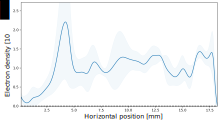
\includegraphics[height=0.3\columnwidth]{DensityLineoutAnnotated.pdf}\hspace{0.5em}%
\includegraphics[height=0.3\columnwidth]{PrettyPic_linICS_Density.pdf}
\caption[Interferometrically measured electron density of the plasma channel and plasma channel emitting recombination light.]{Left: Electron density in electrons per $\mathrm{cm}^{-3}$ in the plasma channel across the gas jet from 0 to 15 mm as measured interferometrically for a range of shots with the blade at the leading edge an without the scattering beam. Right: Plasma channel emitting recombination light, with the laser propagating from left to right. The indicated regions of brighter plasma emission show an increase in the electron density which are consistent with the retrieved electron density profile.}
\label{linICS:Figs:DensityJet}
\end{figure}


A more extensive study and in particular a systematic scan in timing and position of the interaction plane would help to understand this behaviour better.
At the same time this indicates an interesting application of inverse Compton scattering to diagnose the electron beam dynamic in the plasma at the end of the accelerator. Assuming the laser beam does not perturb the plasma significantly and both lasers arrive within a sufficiently small time window, scans in time could be used to investigate the orientation of the momentum vectors in the bubble as it approaches the end of the accelerator and to determine when and how the final momentum distribution, which is measured with the magnetic spectrometer, is frozen into the beam. 

On the other hand, this analysis further re-affirms the hypothesis that the beam properties change throughout its propagation through the remaining plasma. In order to reflect the parameters of the final electron beam the interaction has to occur outside the plasma when the beam fully evolved.

\section{Conclusion}

In this Chapter we presented experimental results from an all-optical colliding pulse setup. We successfully collided relativistic electron beams from a laser wakefield accelerator of up to $1.3\GeV$ energy, injected by a density modulation, with a second laser pulse of intensities between $a_0\sim0.2-1.0$. The laser-electron interaction consistently produced collimated gamma-ray beams from linear inverse Compton scattering. Due to the variability of the electron beams produced in this setup the spectral shape of the gamma radiation varied similarly ranging from narrow-band to broadband radiation of a few MeV to photon energies in excess of $30\MeV$. The radiation was used to diagnose the properties of the laser and the electron beam.

In Section \ref{Chap:linICS:Sec:RasterScan} it was demonstrated that by translating the laser beam relative to the fixed electron beam axis (spatial correlation technique) we can infer the diameter of the laser pulse and, as a result, its intensity at the plane of the interaction, and in turn determining the plane of the interaction.
In Section \ref{Chap:linICS:Sec:YieldBeamSize}, on the other hand, the radiation yield measured on the gamma profile diagnostic was used to infer the diameter and intensity of the laser pulse at the interaction in a single shot. 
Both techniques promise to become useful diagnostics in radiation reaction studies to systematically enable high-intensity interactions by identifying the relative spatio-temporal synchronisation of the electron beam and the laser pulse, but also by allowing a characterisation of the spatio-temporal fluctuations of the laser pulse and the electron beam rather than laser-laser variations that can be characterised, for instance, using spectral interferometry.
\vspace{\baselineskip}

In Section \ref{Chap:linICS:Sec:ICS_EbeamDiag} we then discussed the application of linear inverse Compton scattering as single-shot non-invasive electron beam diagnostic.
The divergence measured from the gamma profile screen and the divergence of the electron beam in the non-dispersion axis were consistent with each other and the gamma profile measurement was then used to infer the ellipticity of the electron beam. 
The ability to measure the ellipticity of the radiation profile and the electron beam, and to separate the two quantities, is in particular useful in the context of intensity measurements in highly non-linear inverse Compton scattering. Here the ellipticity indicates the intensity of the interaction but is convoluted with fluctuations in the electron beam ellipticity \cite{HarShemesh2012_INTENSITY,Yan2017_ICS,Blackburn2019_ModelIndependentLaser}. A statistical characterisation of the transverse electron beam fluctuations will improve the statistical significance and the accuracy of an intensity measurement based on the ellipticity of the gamma emission.
The measured radiation profile also resolved spatial features in the electron beam, for instance smaller off-axis beamlets, and was used to retrieve information on the spatial distribution of the beam in both transverse dimensions, including the dispersion axis that is not spatially resolved in the magnetic spectrometer. 

A lack of correlation in the pointing of the electron bunch and the gamma beam as well as an inversion of the measured gamma radiation to the electron charge distribution indicated that the electron beam properties were evolving between the interaction with the laser pulse and the end of the accelerator. 
This suggests that the radiation from linear inverse Compton scattering will only be a useful final beam diagnostic for divergence, beam pointing and its spatial distribution if the plane of the interaction is outside of the plasma. 
However, it also implies that linear ICS can be applied to investigate the beam evolution and dynamic in the plasma at the end of the accelerator until it reaches its final properties.
\vspace{\baselineskip}

In summary, we demonstrated that linear inverse Compton scattering can act as a useful non-invasive diagnostic of both laser and electron beam properties in multi or single-shot techniques, and will be particularly crucial to enable and properly diagnose high-intensity electron-laser collisions and their statistical variations in future radiation reaction studies.